
\documentclass[11pt]{report}
\usepackage[a4paper,margin=1.5cm]{geometry}
\usepackage[T1]{fontenc}
\usepackage[utf8]{inputenc}
\usepackage{lmodern}
\usepackage{microtype}
\usepackage{amsmath,amssymb,amsfonts,bm,mathtools}
\usepackage{booktabs,tabularx,array,multirow,longtable}
\usepackage{enumitem}
\usepackage{graphicx}
\usepackage{float}
\usepackage{listings}
\usepackage{tikz}
\usetikzlibrary{arrows.meta,positioning,calc,fit,backgrounds,shapes.geometric}
\usepackage[dvipsnames]{xcolor}
\usepackage[hidelinks]{hyperref}
\usepackage[numbers,sort&compress]{natbib}
\usepackage{caption}
\captionsetup{font=small,labelfont=bf}
\setlength{\columnsep}{0.42cm}
\setlength{\parindent}{0pt}
\setlength{\parskip}{2.4pt}
\setlist[itemize]{leftmargin=1.05em,itemsep=1pt,topsep=2pt}
\setlist[enumerate]{leftmargin=1.2em,itemsep=1pt,topsep=2pt}
\renewcommand{\arraystretch}{1.11}
\newcommand{\SO}{\mathrm{SO}(3)}
\newcommand{\SE}{\mathrm{SE}(3)}
\newcommand{\Sthree}{\mathbb{S}^3}
\newcommand{\soLie}{\mathfrak{so}(3)}
\newcommand{\seLie}{\mathfrak{se}(3)}
\newcommand{\veeop}{\operatorname{vee}}
\newcommand{\R}{\mathbb{R}}
\newcommand{\Xspace}{\mathcal{X}}
\newcommand{\Gspace}{\Gamma_T}
\newcommand{\Exp}{\operatorname{Exp}}
\newcommand{\Log}{\operatorname{Log}}
\newcommand{\Cov}{\operatorname{Cov}}
\newcommand{\diag}{\operatorname{diag}}
\newcommand{\Law}{\operatorname{Law}}
\newcommand{\E}{\mathbb{E}}
\newcommand{\argmin}{\operatorname*{argmin}}
\newcommand{\tr}{\operatorname{tr}}
\newcommand{\NIS}{\operatorname{NIS}}
\newcommand{\NEES}{\operatorname{NEES}}
\newcommand{\Normal}{\mathcal{N}}
\newcommand{\se}{\mathfrak{se}}
\newcommand{\norm}[1]{\left\lVert #1 \right\rVert}
\newcommand{\tran}{^{\mathsf T}}
\newcommand{\crossmat}[1]{\left[#1\right]_{\times}}
\newcommand{\Half}{\tfrac12}
\newcommand{\vect}[1]{\boldsymbol{#1}}
\definecolor{Accent}{HTML}{163A63}
\definecolor{Soft}{HTML}{EEF4FA}
\definecolor{Soft2}{HTML}{F8FAFC}
\tikzset{
reportbox/.style={draw=Accent, thick, rounded corners=1.4mm, fill=Soft, align=center, inner sep=4pt},
reportsoft/.style={draw=Accent!70, thick, rounded corners=1.4mm, fill=Soft2, align=center, inner sep=4pt},
reportstate/.style={draw=Accent, thick, rounded corners=1.4mm, fill=blue!8, align=center, inner sep=3pt},
reportmap/.style={draw=Accent, thick, rounded corners=1.4mm, fill=green!12, align=center, inner sep=3pt},
reportfactor/.style={draw=Accent!80, thick, rounded corners=1.2mm, fill=orange!12, align=center, inner sep=2.5pt},
reportarrow/.style={->, thick, draw=Accent},
reportdash/.style={->, semithick, dashed, draw=Accent!75}
}
\lstset{basicstyle=\ttfamily\footnotesize,breaklines=true,frame=single,framesep=4pt,backgroundcolor=\color{Soft2}}
\newcolumntype{Y}{>{\raggedright\arraybackslash}X}
\newcommand{\NotationTable}[1]{%
\vspace{0.6mm}
{\scriptsize
\setlength{\tabcolsep}{2.5pt}
\begin{tabularx}{\columnwidth}{>{\raggedright\arraybackslash}p{0.34\columnwidth}Y}
\toprule
\textbf{New notation} & \textbf{Meaning}\\
\midrule
#1\\
\bottomrule
\end{tabularx}}
\vspace{0.8mm}}
\newcommand{\BigNotationTable}[1]{%
\vspace{0.6mm}
{\scriptsize
\setlength{\tabcolsep}{3.0pt}
\begin{tabularx}{\textwidth}{>{\raggedright\arraybackslash}p{0.17\textwidth}Y>{\raggedright\arraybackslash}p{0.17\textwidth}}
\toprule
\textbf{Symbol} & \textbf{Meaning} & \textbf{How it is used}\\
\midrule
#1\\
\bottomrule
\end{tabularx}}
\vspace{0.8mm}}
\setcounter{secnumdepth}{2}
\setcounter{tocdepth}{2}
\title{Online Bayesian Inversion for an Anchored Multi-Tag Visual--Inertial Rig\\[-1mm]\large Foundations, inference structure, and practical implementation\\[1mm]\normalsize Geometry, priors, likelihoods, estimator hierarchy, and prior-sampling illustrations}
\author{}
\date{}
\graphicspath{{figures/}}


\begin{document}

\hypersetup{pageanchor=false}
\maketitle
\pagenumbering{roman}
\vspace{-6mm}

\begin{abstract}
This report develops an online Bayesian treatment of trajectory and pose estimation for a rigid body carrying a camera and an IMU in an anchored multi-tag environment. One fiducial tag fixes the world frame, while the remaining tags are stationary but initially unknown. The reference model is a posterior on a continuous trajectory together with a static tag map and visual nuisance terms. Practical real-time estimators are then derived as structured approximations: a visual front-end converts tag pixels into pose pseudo-measurements and map updates, while a recursive or fixed-lag visual--inertial back-end propagates and corrects the body state in local coordinates on $\SO$ and $\SE$. The report explains Lie-group state representation, tangent-space Gaussians, quaternion storage versus local error coordinates, curve priors and their discrete state-space forms, pixel-level and pseudo-measurement likelihoods, frame-dependent visual covariance, tag initialization and maintenance, and the exact-versus-approximate treatment of first-frame setup, new-tag birth, and tag reappearance. It closes with parameter guidance, implementation architecture, probabilistic failure modes, and an appendix of prior samples that visualize the motion assumptions encoded by the model.
\end{abstract}

\tableofcontents
\clearpage
\hypersetup{pageanchor=true}
\pagenumbering{arabic}

\chapter{Foundations and Problem Setup}

\begin{table}[t]
\centering
\scriptsize
\setlength{\tabcolsep}{3.0pt}
\begin{tabularx}{\textwidth}{p{0.16\textwidth}p{0.28\textwidth}X}
\toprule
\textbf{Notation} & \textbf{Meaning} & \textbf{Interpretation used in this note}\\
\midrule
$\bar x(t)$ & Continuous-time unknown state curve & The mathematically primary unknown; the prior is a probability law on the whole curve, not only on one sampled state.\\
$x_k$ & Discrete-time sampled state at time $t_k$ & The state used by an online filter after discretization.\\
$\widetilde y$ & Direct noisy sensor reading & We use a tilde for raw sensor measurements such as IMU packets or detected pixels.\\
$\widehat x$ & Estimate or pseudo-measurement & We use a hat for quantities inferred from another inverse problem, e.g. the camera pose estimate delivered by the visual front-end.\\
$\delta x$ & Small local perturbation or error state & The coordinates in which Gaussian priors and Gaussian posteriors are written in EKF/IEKF-type approximations.\\
$T_{AB}$ & Pose of frame $B$ expressed in frame $A$ & It maps coordinates from frame $B$ to frame $A$; $R_{AB}$ and $p_{AB}$ are its rotation and translation blocks.\\
$T_1,T_2$ & Generic elements of $\SE$ & Used when discussing generic pose composition or relative pose error.\\
$A^{-1},A^{\tran}$ & Inverse and transpose & For poses, $T^{-1}$ is the inverse rigid motion; for matrices, $A^{\tran}$ is the transpose.\\
$\Exp,\Log$ & Exponential and logarithm maps & They move between a Lie group such as $\SO$ or $\SE$ and local vector coordinates in its tangent space / Lie algebra.\\
$[\cdot]_{\times}$ and $(\cdot)^\wedge$ & Skew / twist operators & They convert vectors in $\R^3$ or $\R^6$ into matrix form so that group updates can be written by matrix exponentials.\\
$q\in\Sthree$ & Unit quaternion & Alternative representation of orientation. In filtering one usually stores $q$ but keeps covariance on a 3D local rotation error, not on the four quaternion coordinates.\\
$Y_k$ & Raw visual data at frame $k$ & Detected tag corners, tag ids, and per-corner quality information.\\
$z_k^v=(\widehat T_{WC,k},R_{v,k})$ & Visual pose pseudo-measurement & The quantity actually fused by the Bayesian filter in the reduced two-stage architecture.\\
$M=\{T_{WT_j}\}$ & Static map of auxiliary tags & Unknown but stationary non-anchor tag poses; estimated jointly in the full visual inverse problem or by a front-end map-maintenance module.\\
\bottomrule
\end{tabularx}
\caption{Global notation and decoration conventions. This table is meant to make the rest of the note readable without having to infer the meaning of hats, tildes, transform indices, or Lie-group operators from context.}
\end{table}



\section{Geometry, notation, and state representation}
\NotationTable{
$\R^n$ & Euclidean vector space. Positions, velocities, biases, and local error coordinates live in some $\R^n$.\\
$\SO$ & Rotation group in 3D. Elements are proper orthogonal matrices and represent orientation.\\
$\SE$ & Rigid-motion group in 3D. Elements represent a full pose made of rotation and translation.\\
$\soLie,\seLie$ & Lie algebras / tangent spaces associated with $\SO$ and $\SE$.\\
$\Sthree$ & Unit-quaternion manifold. A quaternion $q\in\Sthree$ is another way to represent a rotation.\\
$\Pi_0$ & Prior law on the unknown trajectory curve.\\
$\widehat{\cdot},\widetilde{\cdot},\bar{\cdot},\delta(\cdot)$ & Estimated quantity, direct noisy measurement, whole curve, and local perturbation / error-state notation.}

This opening section fixes the geometric language used throughout the report. Positions, velocities, and sensor biases are Euclidean variables, but orientations and rigid poses are not. The estimator therefore mixes ordinary vectors with manifold-valued states, and all later priors, residuals, and covariance statements inherit that choice.

\subsection{Euclidean variables versus pose variables}
\NotationTable{
$p,v,b_g,b_a\in\R^3$ & Position, velocity, gyroscope bias, and accelerometer bias.\\
$R\in\SO$ & Rotation matrix.\\
$T=\begin{bmatrix}R&p\\0&1\end{bmatrix}\in\SE$ & Homogeneous rigid transform.\\
$W,B,C$ & World, body/IMU, and camera frames.}

A vector in $\R^3$ can be added, subtracted, and averaged directly. For example, if $p_1,p_2\in\R^3$ are two positions, then $p_2-p_1$ is another vector in $\R^3$. This is why Gaussians on positions or velocities are straightforward.

A rotation is different. The set of all valid 3D rotations is
\begin{equation}
\SO=\{R\in\R^{3\times 3}:R\tran R=I,\ \det R=1\}.
\end{equation}
This is not a linear vector space: if $R_1,R_2\in\SO$, then the arithmetic average $\tfrac12(R_1+R_2)$ is usually \emph{not} a valid rotation matrix. Similarly, a full rigid pose belongs to
\begin{equation}
\SE=\left\{\begin{bmatrix}R&p\\0&1\end{bmatrix}:R\in\SO,\ p\in\R^3\right\},
\end{equation}
which is again not a linear space. This is the reason that pose errors in the rest of the note are written through relative transforms and logarithms, not by subtracting the entries of two $4\times4$ matrices.

The transform convention used throughout the note is the robotics convention
\begin{equation}
T_{AB}=\begin{bmatrix}R_{AB}&p_{AB}\\0&1\end{bmatrix},
\end{equation}
meaning ``pose of frame $B$ expressed in frame $A$.'' If a point has coordinates $x_B$ in frame $B$, then its coordinates in frame $A$ are
\begin{equation}
\begin{bmatrix}x_A\\1\end{bmatrix}=T_{AB}\begin{bmatrix}x_B\\1\end{bmatrix}.
\end{equation}
Thus $T_{AB}^{-1}=T_{BA}$. When the notation $T_1,T_2$ is used later, it simply means generic poses in $\SE$ without specifying their frame labels.

\subsection{Lie groups, operations, and local coordinates}
\NotationTable{
$\soLie$ & Tangent space of $\SO$ at the identity. It consists of $3\times3$ skew-symmetric matrices.\\
$\seLie$ & Tangent space of $\SE$ at the identity. It is the 6D space of twists.\\
$[\phi]_{\times}$ & Skew-symmetric matrix built from $\phi\in\R^3$.\\
$\xi^\wedge$ & Matrix form of a pose perturbation $\xi\in\R^6$.\\
$\Exp,\Log$ & Maps between the group and local vector coordinates.\\
$\phi,\xi$ & Local rotation error and local pose error coordinates.}

A Lie group is a smooth manifold equipped with globally valid group operations. In this report the concrete Lie groups are $\SO$ for orientation and $\SE$ for full rigid pose. What matters in practice is that one can compose and invert poses globally, while still doing calculus and Gaussian approximation in a local vector space. That local vector space is the tangent space at the identity, also called the Lie algebra.

\begin{center}
{\scriptsize
\setlength{\tabcolsep}{4pt}
\begin{tabular}{p{0.20\columnwidth}p{0.27\columnwidth}p{0.41\columnwidth}}
\toprule
\textbf{Operation} & \textbf{Example} & \textbf{Why it appears later}\\
\midrule
Identity & $I\in\SO,\ I_4\in\SE$ & reference element for local coordinates and perturbations\\
Composition & $R_1R_2,\ T_1T_2$ & chaining body, camera, and tag poses\\
Inverse & $R^{-1}=R\tran,\ T^{-1}$ & frame changes and relative transforms\\
Exponential map & $\Exp([\phi]_\times),\ \Exp(\xi^\wedge)$ & injecting local updates back onto the manifold\\
Logarithm map & $\Log(R_1^{-1}R_2),\ \Log(T_1^{-1}T_2)$ & writing residuals in local coordinates\\
Retraction & $T^+=T\Exp(\xi^\wedge)$ & EKF, IEKF, and Gauss--Newton correction steps\\
\bottomrule
\end{tabular}}
\end{center}

For rotations, the Lie algebra is
\begin{equation}
\soLie=\{\Omega\in\R^{3\times3}:\Omega\tran=-\Omega\}.
\end{equation}
Every vector $\phi=[\phi_1\ \phi_2\ \phi_3]\tran\in\R^3$ corresponds to a skew-symmetric matrix
\begin{equation}
[\phi]_{\times}=\begin{bmatrix}
0 & -\phi_3 & \phi_2\\
\phi_3 & 0 & -\phi_1\\
-\phi_2 & \phi_1 & 0
\end{bmatrix}.
\label{eq:skew_definition_sweep}
\end{equation}
This is why $\R^3$ is used as the minimal local coordinate system for small rotation errors. A small orientation perturbation $\delta\theta\in\R^3$ updates a nominal rotation by
\begin{equation}
R^+=R\,\Exp([\delta\theta]_{\times}).
\label{eq:rotation_update_sweep}
\end{equation}
For a full pose, the local perturbation is a twist
\begin{equation}
\xi=\begin{bmatrix}\rho\\ \phi\end{bmatrix}\in\R^6,
\end{equation}
with matrix form
\begin{equation}
\xi^\wedge=\begin{bmatrix}[\phi]_{\times} & \rho\\ 0 & 0\end{bmatrix}\in\seLie.
\label{eq:wedge_definition_sweep}
\end{equation}
Then a pose update is written as
\begin{equation}
T^+=T\,\Exp(\xi^\wedge).
\label{eq:pose_update_sweep}
\end{equation}
The logarithm map does the reverse: it converts a small relative transform into local vector coordinates. For two poses $T_1,T_2\in\SE$, the relative pose error is
\begin{equation}
\xi=\Log(T_1^{-1}T_2)\in\R^6.
\label{eq:relative_pose_error_log_sweep}
\end{equation}
This is the mathematically correct replacement for ``$T_2-T_1$'' when the unknown is a rigid pose. Throughout the report we use this same right-multiplicative convention: nearby poses are represented as $T=\widehat T\Exp(\xi^\wedge)$, and local residuals are written with the corresponding right-invariant relative transform.

This machinery cannot be avoided in the present problem. A Gaussian density such as $\mathcal N(m,P)$ is defined on a vector space, not on a curved manifold. Therefore the posterior over orientation or pose cannot literally be represented as a Gaussian over the raw entries of $R$, $T$, or a quaternion while still respecting the rotation constraints. The standard construction is to keep the \emph{nominal state} on the manifold but represent uncertainty in local Euclidean coordinates. In other words, the posterior is approximated by
\begin{equation}
T = \widehat T\,\Exp(\xi^\wedge),
\qquad
\xi\sim\mathcal N(0,P_T),
\end{equation}
or, for orientation alone,
\begin{equation}
R = \widehat R\,\Exp([\delta\theta]_{\times}),
\qquad
\delta\theta\sim\mathcal N(0,P_R).
\end{equation}
Lie groups are therefore not cosmetic notation. They are what keeps composition, residuals, linearization, and Gaussian uncertainty mutually consistent. The same local-coordinate language reappears in the trajectory prior, in visual residuals, in the EKF error state, and in factor-graph updates \citep{sola2018micro,barrau2017invariant}.

\subsection{Quaternions: storage choice, same local geometry}
\NotationTable{
$q=[q_w\ q_x\ q_y\ q_z]\tran$ & Quaternion written as one scalar part and a 3D vector part.\\
$q\in\Sthree$ & Unit quaternion satisfying $\norm{q}=1$.\\
$q\sim -q$ & Double-cover property: $q$ and $-q$ represent the same physical rotation.\\
$\otimes$ & Quaternion product.\\
$\delta q$ & Small quaternion correction built from a 3D local rotation error.}

Many implementations do not store a rotation matrix directly. They store a unit quaternion
\begin{equation}
q\in\Sthree=\{q\in\R^4:\norm{q}=1\}.
\end{equation}
Quaternions are a convenient storage format: they are compact, easy to normalize, and easy to propagate numerically. They do \emph{not}, however, turn orientation into an ordinary 4D Euclidean state. A quaternion has a unit-norm constraint and the sign ambiguity $q\sim -q$, since both represent the same element of $\SO$.

For that reason, good filters do \emph{not} place a naive 4D Gaussian directly on the quaternion coordinates. They follow exactly the same local-coordinate construction as with rotation matrices: the state stores a nominal quaternion $\widehat q$, while uncertainty lives in a 3D rotation error $\delta\theta\in\R^3$. A small correction is converted into a unit quaternion; to first order one may write
\begin{equation}
\delta q \approx \begin{bmatrix}1\\ \Half\delta\theta\end{bmatrix}
\quad\text{for small }\delta\theta,
\end{equation}
and the nominal quaternion is updated consistently with the right-multiplicative convention above, e.g.
\begin{equation}
q^+ = q\otimes \delta q.
\label{eq:quat_update_sweep}
\end{equation}
The quaternion representation is therefore subordinate to the Lie-group story, not a competing alternative to it. One stores orientation by a unit quaternion for convenience, but Bayesian linearization, covariance propagation, and Kalman correction still live in a 3D tangent coordinate. This is the standard multiplicative-quaternion or error-state-quaternion viewpoint \citep{sola2017quaternion,sola2018micro}.

\subsection{Why the unknown is really a random curve}
\NotationTable{
$\bar x(t)$ & Continuous-time trajectory state.\\
$\Gspace$ & Admissible set of such curves on $[0,T]$.\\
$\Pi_0$ & Prior law on the curve.}

The unknown in trajectory estimation is not a single pose and not a single finite vector. It is a time-indexed object: a curve that assigns a state to every time $t\in[0,T]$. The mathematically clean Bayesian object is therefore a probability measure on a path space. In this report the continuous-time state is written as
\begin{equation}
\bar x(t)=\big(R(t),p(t),v(t),\omega(t),b_g(t),b_a(t)\big),
\end{equation}
where orientation is manifold-valued and the remaining variables are Euclidean. A convenient admissible path space is
\begin{equation}
\begin{aligned}
\Gspace=\Bigl\{\bar x:[0,T]\to \SO\times(\R^3)^5\;\Big|\;
&v,\omega,b_g,b_a\in C([0,T]),\\
&p,R\text{ are absolutely continuous},\\
&\dot p=v,\ \dot R=R[\omega]_{\times}\ \text{a.e.}\Bigr\}.
\end{aligned}
\end{equation}
The exact function-space choice is not the main point. The point is that the prior $\Pi_0$ is defined on whole curves and encodes which trajectories are plausible before any data are seen \citep{stuart2010inverse,hairer2007bayesian}.

\begin{figure}[t]
\centering
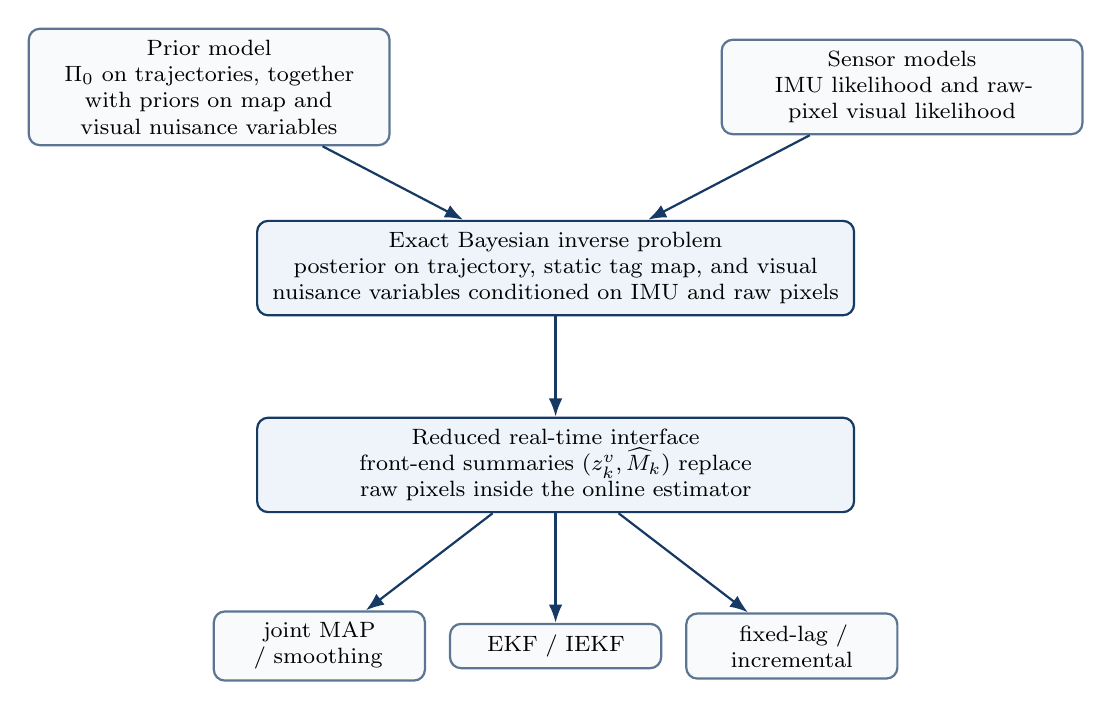
\begin{tikzpicture}[font=\footnotesize, >=Latex, x=1cm, y=1cm]
  \node[reportsoft, text width=4.3cm] (prior) at (0,0) {Prior model\\$\Pi_0$ on trajectories, together with priors on map and visual nuisance variables};
  \node[reportsoft, text width=4.3cm] (data) at (8.8,0) {Sensor models\\IMU likelihood and raw-pixel visual likelihood};
  \node[reportbox, text width=7.3cm] (full) at (4.4,-2.3) {Exact Bayesian inverse problem\\posterior on trajectory, static tag map, and visual nuisance variables conditioned on IMU and raw pixels};
  \node[reportbox, text width=7.3cm] (reduced) at (4.4,-4.8) {Reduced real-time interface\\front-end summaries $(z_k^v,\widehat M_k)$ replace raw pixels inside the online estimator};
  \node[reportsoft, text width=2.4cm] (joint) at (1.4,-7.1) {joint MAP / smoothing};
  \node[reportsoft, text width=2.4cm] (filter) at (4.4,-7.1) {EKF / IEKF};
  \node[reportsoft, text width=2.4cm] (lag) at (7.4,-7.1) {fixed-lag / incremental};
  \draw[reportarrow] (prior) -- (full);
  \draw[reportarrow] (data) -- (full);
  \draw[reportarrow] (full) -- (reduced);
  \draw[reportarrow] (reduced) -- (joint);
  \draw[reportarrow] (reduced) -- (filter);
  \draw[reportarrow] (reduced) -- (lag);
\end{tikzpicture}
\caption{Conceptual hierarchy. The reference model is a posterior on trajectory, map, and nuisance variables; the real-time estimator works with condensed front-end summaries and then approximates that reduced problem numerically.}
\end{figure}

\section{Problem setup and measurement interface}
\NotationTable{
$W,B,C$ & World, body/IMU, and camera coordinate frames.\\
$y^u$ & Entire IMU data stream over $[0,T]$.\\
$Y_k$ & Raw image-side data at frame $k$, i.e. detected tag corners and quality metadata.\\
$z^v_k$ & Visual pose pseudo-measurement delivered to the Bayesian filter; here $z^v_k=(\widehat T_{WC,k},R_{v,k})$.\\
$\widehat T_{WC,k}$ & Estimated camera pose in the world frame at frame time $t_k$.\\
$R_{v,k}$ & Covariance of the visual pose pseudo-measurement.\\
$\mathcal J_{\mathrm{aux}}$ & Index set of non-anchor tags whose world poses are unknown but stationary.\\
$M$ & Static auxiliary-tag map $M=\{T_{WT_j}\}_{j\in\mathcal J_{\mathrm{aux}}}$.\\
$T_{BC}$ & Known rigid transform from IMU/body frame to camera frame.}

We assume a rigid body carrying an IMU and a camera. The world frame $W$ is anchored by at least one known calibration pattern. In the multi-tag case emphasized later, tag $j=0$ is the anchor and its world pose $T_{WT_0}$ is known (often chosen as the identity pose), while the remaining tags $j\in\mathcal J_{\mathrm{aux}}$ are only known to be stationary. The IMU/body frame is $B$, the camera frame is $C$, and the rigid body-to-camera transform
\begin{equation}
T_{BC}=\begin{bmatrix}R_{BC}&t_{BC}\\0&1\end{bmatrix}\in\SE
\end{equation}
is assumed known from an earlier calibration step.

Two data streams are available. First, the IMU outputs angular-rate and specific-force measurements, collected at high rate. Second, every video frame provides an image of the anchor tag and possibly auxiliary stationary tags. In this chapter the raw pixels are \emph{not} fused directly into the Bayesian trajectory estimator. Instead, the visual front-end solves an image-side inverse problem and passes the output
\begin{equation}
z^v_k=(\widehat T_{WC,k},R_{v,k})
\end{equation}
into the Bayesian filter. This separation matters: the online inverse problem solved by the filter uses pose pseudo-measurements, while the raw pixels still influence the filter indirectly through the frame-dependent covariance $R_{v,k}$ and, in the multi-tag case, through the current estimate of the auxiliary-tag map $M$.

Formally, the raw visual data at frame $k$ are
\begin{equation}
Y_k=\{\widetilde u_{i,k}^{(j)},\ s_{i,k}^{(j)},\ \text{tag id }j\}_{j\in\mathcal V_k,\ i=1,\dots,m_j},
\end{equation}
where $\widetilde u_{i,k}^{(j)}\in\R^2$ is the detected pixel coordinate of corner $i$ of tag $j$, $s_{i,k}^{(j)}$ denotes detector quality metadata such as margin or score, and $\mathcal V_k$ is the set of visible tags at frame $k$. In the simplest anchor-only case the front-end computes
\begin{equation}
(\widehat T_{WC,k},R_{v,k})=\mathcal G_k(Y_k).
\end{equation}
In the more realistic case with unknown but stationary auxiliary tags, the front-end is better written as
\begin{equation}
(\widehat T_{WC,k},R_{v,k},\widehat M_k)=\mathcal G_k(Y_{0:k}),
\end{equation}
meaning that the current pose estimate may depend on all raw visual data seen so far through a recursively updated map estimate $\widehat M_k$. The full Bayesian inverse problem is then naturally posed on $(\bar x,M)$, whereas the reduced online filter described in this chapter conditions on the condensed visual output and typically treats the current map estimate as an external input. In symbols, the reduced filter solves
\begin{equation}
\Pi(d\bar x\mid y^u,z^v,\widehat M),
\end{equation}
not directly $\Pi(d\bar x,dM\mid y^u,Y)$.

This two-stage architecture is common in practice because it decouples the hard image-processing problem from the state-estimation problem. The price is that the visual part of the filter must be given a realistic covariance model, and the map-maintenance module must be kept conceptually separate from the recursive state estimator. If $R_{v,k}$ is too small, the filter will over-trust the pose front-end. If it is too large, the filter will behave almost like dead reckoning between occasional visual corrections.

\subsection{How the literature instantiates the same inverse problem}
\NotationTable{
Markov prior & Prior that factorizes as $p(x_0)\prod_k p(x_{k+1}\mid x_k)$.\\
GP prior & Gaussian-process prior on the whole continuous-time trajectory curve.\\
MAP & Maximum a posteriori estimate: the minimizer of the negative log posterior.\\
Fixed lag & Approximate smoothing over a moving recent time window.}

The state of the art differs mainly in \emph{how the prior over trajectories is represented} and \emph{how the posterior is approximated}. Path-space Bayesian inversion papers treat the unknown as a random function or path and define the posterior directly on that function space; Stuart gives the general inverse-problem treatment, and Apte et al.\ make the path-space viewpoint explicit for data assimilation \citep{stuart2010inverse,hairer2007bayesian}. Classical recursive Bayesian tracking assumes a discrete-time Markov prior and performs prediction and update sequentially; EKF, UKF, and particle filters are all approximations to this same recursive posterior \citep{arulampalam2002particle,sarkka2023bayesian}. Filter-based visual--inertial odometry, exemplified by MSCKF and related consistency-focused filter formulations, uses recursive filtering with inertial propagation and visual correction \citep{mourikis2007msckf,hesch2014consistency,yang2022dri}. Optimization-based methods such as OKVIS, IMU preintegration methods, and iSAM2 represent the posterior through a negative log posterior and solve it by sliding-window or incremental nonlinear optimization \citep{leutenegger2015okvis,forster2017preintegration,kaess2012isam2}. Continuous-time trajectory methods use GP priors generated by stochastic differential equations and then perform batch GP regression / smoothing on the curve \citep{anderson2015gp,dong2017sparsegp}.

\begin{table}[t]
\centering
\scriptsize
\setlength{\tabcolsep}{3.4pt}
\begin{tabularx}{\textwidth}{p{0.14\textwidth}p{0.17\textwidth}p{0.23\textwidth}p{0.17\textwidth}X}
\toprule
\textbf{Representative work} & \textbf{Unknown object} & \textbf{Prior / regularizer} & \textbf{Inference style} & \textbf{What it assumes or emphasizes}\\
\midrule
Stuart (2010) \citep{stuart2010inverse} & Function or curve in infinite-dimensional space & Prior measure on the whole unknown, often Gaussian on a function space & Full Bayesian posterior on the unknown space & General Bayesian inverse viewpoint; emphasizes posterior well-posedness and priors on spaces of functions.\\
Apte et al. (2007) \citep{hairer2007bayesian} & Continuous-time path & Path-space prior induced by model dynamics and noise & MCMC / path-space Bayesian assimilation & Explicitly formulates data assimilation as conditioning a probability law on paths.\\
Arulampalam et al. (2002) \citep{arulampalam2002particle} & Discrete state trajectory & Markov state-transition prior & Recursive Bayesian filtering, including particle filters & Generic nonlinear / non-Gaussian online Bayesian tracking.\\
Mourikis--Roumeliotis (2007) \citep{mourikis2007msckf} & Pose, velocity, biases, camera clones & IMU-driven Gaussian Markov prior with bias random walks & EKF / MSCKF & Real-time vision-aided inertial navigation with recursive updates.\\
Leutenegger et al. (2015) \citep{leutenegger2015okvis} & Keyframe poses, velocities, biases, landmarks & Gaussian priors plus IMU factors and robust visual residuals & Nonlinear MAP / fixed-lag optimization & Tightly coupled VIO with sliding-window refinement.\\
Forster et al. (2017) \citep{forster2017preintegration} & Keyframe states plus preintegrated increments & Discrete Gaussian motion prior expressed by on-manifold IMU factors & MAP / factor graph / incremental smoothing & Efficient manifold-correct inertial factors and delayed bias correction.\\
Anderson--Barfoot--Tong--S{\"a}rkk{\"a} (2015) \citep{anderson2015gp} & Entire continuous-time trajectory curve & GP prior generated by a linear time-varying SDE & Batch GP regression / smoothing & Continuous-time prior, interpolation at arbitrary times, exact sparsity.\\
\bottomrule
\end{tabularx}
\caption{Representative Bayesian formulations for trajectory-pose estimation. The same problem can be expressed through path-space priors, discrete Markov priors, MAP objectives, or continuous-time Gaussian-process priors.}
\end{table}

\section{Bayesian model for the trajectory prior}
\NotationTable{
$\bar x(t)$ & Continuous-time latent state. In the prior model we use $\bar x(t)=(R(t),p(t),v(t),\omega(t),b_g(t),b_a(t))$.\\
$w_v,w_\omega$ & White-noise drives for translational and rotational smoothness.\\
$w_{bg},w_{ba}$ & White-noise drives for gyro and accelerometer bias drift.\\
$Q_v,Q_\omega,Q_{bg},Q_{ba}$ & Spectral-density matrices controlling roughness of the prior.\\
$m_0,P_0$ & Mean and covariance of the initial-state prior.\\
$\Sigma_{\mathrm{map}}$ & Optional prior covariance for a sequence-level visual bias.}

A prior on the curve $\bar x(\cdot)$ must say which trajectories are plausible before seeing the data. In this report the prior is introduced as the law of a stochastic process generated by a stochastic differential equation. This section is the first half of the Bayesian model: it explains the trajectory law before any sensor likelihood is applied. Write
\begin{equation}
\bar x(t)=\big(R(t),p(t),v(t),\omega(t),b_g(t),b_a(t)\big),
\end{equation}
with kinematic relations
\begin{equation}
\dot p(t)=v(t),
\qquad
\dot R(t)=R(t)\crossmat{\omega(t)}.
\end{equation}
A smoothness prior is then generated by
\begin{align}
\dot v(t) &= w_v(t), & w_v(t) &\sim \mathcal N(0,Q_v\,\delta(t-t')),\\
\dot \omega(t) &= w_\omega(t), & w_\omega(t) &\sim \mathcal N(0,Q_\omega\,\delta(t-t')),\\
\dot b_g(t) &= w_{bg}(t), & w_{bg}(t) &\sim \mathcal N(0,Q_{bg}\,\delta(t-t')),\\
\dot b_a(t) &= w_{ba}(t), & w_{ba}(t) &\sim \mathcal N(0,Q_{ba}\,\delta(t-t')).
\label{eq:curve_prior_sde_new}
\end{align}
Under the continuous-time white-noise idealization, these equations are interpreted in integral form and define a probability law $\Pi_0=\mathrm{Law}(\bar x)$ on $\Gspace$. Translational acceleration, angular acceleration, and bias drift are modeled through zero-mean stochastic drives. The matrices $Q_v,Q_\omega,Q_{bg},Q_{ba}$ are therefore not measurement-noise covariances; they are \emph{hyperparameters of the prior law on trajectories}. They control how rough the trajectory is allowed to be. Small $Q_v$ means the prior expects nearly constant velocity. Large $Q_v$ allows aggressive translational maneuvers. Small $Q_{bg}$ and $Q_{ba}$ imply nearly constant biases, while larger values allow faster drift.

A commonly used formal quadratic action associated with this prior is
\begin{equation}
\mathcal J_{\mathrm{prior}}^{\mathrm{formal}}(\bar x)
=\Half\int_0^T \Big(\norm{\dot v}_{Q_v^{-1}}^2+\norm{\dot\omega}_{Q_\omega^{-1}}^2+\norm{\dot b_g}_{Q_{bg}^{-1}}^2+\norm{\dot b_a}_{Q_{ba}^{-1}}^2\Big)dt,
\label{eq:formal_curve_prior_energy}
\end{equation}
subject to the kinematic constraints on $R$ and $p$. Equation~\eqref{eq:formal_curve_prior_energy} should be read as a formal shorthand or MAP/discretized surrogate on admissible paths; it is \emph{not} a literal density of $\Pi_0$ with respect to a path-space Lebesgue measure.

\subsection{Why these prior components are reasonable}
\NotationTable{
$Q_v$ & Controls translational roughness. Large values mean rapid changes of acceleration are plausible.\\
$Q_\omega$ & Controls rotational roughness. Large values mean rapid changes of angular velocity are plausible.\\
$Q_{bg},Q_{ba}$ & Control how quickly gyro and accelerometer biases are allowed to drift.\\
$\rho_p,\rho_R,Q_c$ & Parameters of colored visual-noise state, introduced later.}

The rationale for the prior components is physical. Over short video intervals, position and orientation do not jump discontinuously, so a constant-velocity / constant-angular-velocity prior is a sensible default. The white-noise drives in \eqref{eq:curve_prior_sde_new} provide a simple smoothness model that still admits real maneuvers. Bias random walks are used because MEMS bias drift is slow, cumulative, and not known a priori; a random walk is a common tractable model for a slowly varying nuisance offset and integrates well with filters and smoothers. The same bias-random-walk nuisance model is used in Kalibr and in standard visual--inertial formulations such as MSCKF-style filters and preintegrated optimization methods \citep{kalibr_noise,mourikis2007msckf,forster2017preintegration}.

The prior may also include nuisance terms not tied directly to rigid-body dynamics. A sequence-level visual bias can be represented as
\begin{equation}
 b_{\mathrm{map}}\sim \mathcal N(0,\Sigma_{\mathrm{map}}),
\end{equation}
where $b_{\mathrm{map}}\in\R^6$ captures slowly varying or constant pose offsets due to imperfect anchor geometry, imperfect camera calibration, or tag-model mismatch. If the anchor and camera model are treated as exact, set $b_{\mathrm{map}}=0$.

\subsection{From the curve prior to the state-space prior used by a Kalman filter}
\NotationTable{
$\tilde x_k$ & Sampled extended state at frame time $t_k$, here $\tilde x_k=(R_k,p_k,v_k,\omega_k,b_{g,k},b_{a,k})$.\\
$x_k$ & Reduced practical filter state, usually $x_k=(R_k,p_k,v_k,b_{g,k},b_{a,k})$ after conditioning on IMU packets.\\
$p(\tilde x_{k+1}\mid \tilde x_k)$ & One-step Markov transition induced by the discretized SDE.\\
$\theta_{\mathrm{prior}}$ & Collection of prior hyperparameters.}

A Kalman filter does not manipulate the full path measure directly. A sampled SDE is Markov on an extended state that contains all variables needed to close the dynamics. For the prior above that extended state is
\begin{equation}
\tilde x_k=(R_k,p_k,v_k,\omega_k,b_{g,k},b_{a,k}),
\end{equation}
and its sampled law factorizes as
\begin{equation}
 p(\tilde x_{0:N})=p(\tilde x_0)\prod_{k=0}^{N-1}p(\tilde x_{k+1}\mid \tilde x_k;\theta_{\mathrm{prior}}),
\label{eq:markov_factorization_from_curve}
\end{equation}
and hyperparameter set
\begin{equation}
\theta_{\mathrm{prior}}=\{m_0,P_0,Q_v,Q_\omega,Q_{bg},Q_{ba},\Sigma_{\mathrm{map}},\rho_p,\rho_R,Q_c\}.
\end{equation}
In many practical VIO filters the angular velocity is not carried as a separate state because the gyroscope packets are treated as observed inputs in the propagation step. After conditioning on the IMU packets between frames, one obtains the reduced transition kernel $p(x_{k+1}\mid x_k,\mathcal U_k)$ for
\begin{equation}
 x_k=(R_k,p_k,v_k,b_{g,k},b_{a,k}).
\end{equation}
Thus the Markov prior used by a filter is not a different physical prior; it is a sampled and, if desired, measurement-conditioned form of the same prior-on-curves.

A convenient initial prior is specified locally around a nominal initial state $m_0$: rotational components are perturbed multiplicatively, Euclidean components additively, and the local error covariance is $P_0$. The nominal state $m_0$ is usually derived from the first reliable visual pose, a short stationary IMU segment, or trusted setup geometry, and $P_0$ expresses how uncertain that initialization is. A common block structure is
\begin{equation}
P_0=\diag(\sigma_{R0}^2I_3,\sigma_{p0}^2I_3,\sigma_{v0}^2I_3,\sigma_{bg0}^2I_3,\sigma_{ba0}^2I_3).
\end{equation}


\subsection{Prior for stationary but initially unknown auxiliary tags}
\NotationTable{
$M=\{T_{WT_j}\}_{j\in\mathcal J_{\mathrm{aux}}}$ & Static map of auxiliary tag poses.\\
$\pi_M(M)$ & Prior law on the auxiliary-tag map.\\
$\mathcal W$ & Coarse workspace region in which auxiliary tags are believed to lie.\\
$\mu_{M,j},\Sigma_{M,j}$ & Mean and covariance of a local Gaussian prior for auxiliary tag $j$ after anchored initialization.}

When only one tag is anchored, the prior is not only a law on the body trajectory. It also includes a prior on the unknown but stationary auxiliary-tag map
\begin{equation}
M=\{T_{WT_j}\}_{j\in\mathcal J_{\mathrm{aux}}}.
\end{equation}
Before any anchored observation of auxiliary tag $j$, the mathematically honest prior is broad: we only know that the tag is stationary and that it lies somewhere in the lab workspace. A minimal prior is therefore a support prior of the form
\begin{equation}
\pi_M(dM) \propto \prod_{j\in\mathcal J_{\mathrm{aux}}} \mathbf 1\{p_{WT_j}\in\mathcal W\}\,\pi_{R,j}(dR_{WT_j}),
\label{eq:workspace_prior_aux_tags}
\end{equation}
where $\mathcal W\subset\R^3$ is a coarse workspace box and $\pi_{R,j}$ is an orientation prior reflecting any known mounting convention, for example ``tags are roughly vertical on walls'' or ``tags are roughly horizontal on cube tops.''

Once an auxiliary tag is first seen simultaneously with the anchor, one obtains an anchored initialization $\mu_{M,j}=\widehat T_{WT_j}^{\mathrm{init}}$. After that point the prior can be tightened and written in local Lie coordinates as
\begin{equation}
T_{WT_j}=\mu_{M,j}\Exp(\eta_{M,j}^\wedge),
\qquad
\eta_{M,j}\sim\mathcal N(0,\Sigma_{M,j}),
\label{eq:local_aux_map_prior}
\end{equation}
with small or slowly shrinking covariance $\Sigma_{M,j}$. Again, the Gaussian lives in the local coordinate $\eta_{M,j}\in\R^6$, not directly on $\SE$. In a batch or fixed-lag front-end this is the natural way to represent ``stationary but initially unknown.'' In an online filter, one either augments the state with these nearly-static variables or lets a separate front-end map-maintenance module update $\widehat M_k$ and its uncertainty.

The key conceptual point is that the anchor removes the global $\SE$ gauge freedom, while the stationary auxiliary-tag prior regularizes the remaining map estimation problem. Without the anchor, the camera trajectory and the whole map could drift together by the same rigid transform without changing any pixel prediction.


\section{Bayesian model for the IMU channel}
\NotationTable{
$\widetilde\omega(t)$ & Measured angular velocity.\\
$\widetilde a(t)$ & Measured specific force.\\
$g_W$ & Gravity in the world frame.\\
$n_g,n_a$ & Zero-mean gyro and accelerometer white noise.\\
$b_g,b_a$ & Slowly varying gyro and accelerometer biases.\\
$R_g,R_a$ & Continuous-time gyro and accelerometer noise intensities used in the formal likelihood notation; after discretization they contribute to $Q_k$.}

The IMU returns two signals: angular rate from the gyroscope and specific force from the accelerometer. The gyroscope model is
\begin{equation}
\widetilde\omega(t)=\omega(t)+b_g(t)+n_g(t),
\label{eq:gyro_model_final}
\end{equation}
where $\omega(t)$ is the true angular velocity expressed in the body frame, $b_g(t)$ is a slowly varying bias, and $n_g(t)$ is fast zero-mean noise.

The accelerometer is more subtle. It does not measure world-frame acceleration directly. It measures the non-gravitational specific force expressed in the sensor frame:
\begin{equation}
\widetilde a(t)=R_{BW}(t)\big(\ddot p_W(t)-g_W\big)+b_a(t)+n_a(t).
\label{eq:accel_model_final}
\end{equation}
Here $\ddot p_W(t)$ is translational acceleration in the world frame and $g_W$ is the gravity vector in that same frame. The term $R_{BW}(t)(\ddot p_W(t)-g_W)$ converts the world-frame specific force into body coordinates. This is why inertial propagation later re-adds gravity in the world frame \citep{kok2017inertial,forster2017preintegration}.

\subsection{IMU as a likelihood on the unknown curve}
\NotationTable{
$\Phi_u(\bar x;y^u)$ & IMU negative log-likelihood or data-misfit functional.\\
$\norm{r}_{M^{-1}}^2$ & Weighted squared norm $r\tran M^{-1}r$.}

If one stays in the path-space Bayesian language, the IMU contributes a data-misfit functional on the whole curve. Under the common Gaussian white-noise idealization one writes formally
\begin{equation}
\Phi_u(\bar x;y^u)=\Half\int_0^T\left[\norm{\widetilde\omega(t)-\omega(t)-b_g(t)}_{R_g^{-1}}^2+\norm{\widetilde a(t)-R_{BW}(t)(\ddot p(t)-g_W)-b_a(t)}_{R_a^{-1}}^2\right]dt.
\label{eq:imu_curve_likelihood}
\end{equation}
This is the continuous-time analogue of the familiar sum of weighted squared innovations: for any candidate trajectory curve, it quantifies how well that curve explains the measured angular rates and specific forces. As in the prior section, the white-noise notation is formal; rigorous treatments interpret it through discretization or Gaussian-measure constructions rather than through an ordinary Lebesgue density on signal space.

\subsection{IMU as the process model used by a practical online filter}
\NotationTable{
$\mathcal U_k$ & All IMU packets between $t_k$ and $t_{k+1}$.\\
$Q_k$ & Effective discrete process covariance over one propagation interval.}

In an online filter it is more convenient to condition on the IMU packets and use the resulting state-transition model. The corresponding continuous-time kinematics are
\begin{align}
\dot R_{WB} &= R_{WB}(\widetilde\omega-b_g-n_g)^\wedge,\\
\dot v_{WB} &= g_W + R_{WB}(\widetilde a-b_a-n_a),\\
\dot p_{WB} &= v_{WB},\\
\dot b_g &= w_{bg},\\
\dot b_a &= w_{ba}.
\end{align}
A first-order discrete propagation over one camera interval is
\begin{equation}
R_{k+1}=R_k\Exp\!\big((\widetilde\omega_k-b_{g,k})\Delta t\big),
\end{equation}
\begin{equation}
v_{k+1}=v_k+\big(g_W+R_k(\widetilde a_k-b_{a,k})\big)\Delta t+n_k^v,
\end{equation}
\begin{equation}
p_{k+1}=p_k+v_k\Delta t+\Half\big(g_W+R_k(\widetilde a_k-b_{a,k})\big)\Delta t^2+n_k^p,
\end{equation}
\begin{equation}
b_{g,k+1}=b_{g,k}+n_k^{bg},\qquad b_{a,k+1}=b_{a,k}+n_k^{ba}.
\label{eq:discrete_process_model_final}
\end{equation}
The discrete noise terms above are not independent free parameters; they arise from integrating $n_g,n_a,w_{bg},w_{ba}$ over $[t_k,t_{k+1}]$, and their joint covariance is summarized by $Q_k$. Equation~\eqref{eq:discrete_process_model_final} is therefore a first-order discretization of the IMU-conditioned state transition used in EKF-, IEKF-, or fixed-lag estimators \citep{mourikis2007msckf,forster2017preintegration,barrau2017invariant}.


\section{Bayesian model for the visual channel}
\NotationTable{
$Y_k$ & Raw visual data at frame $k$: detected corners, tag ids, and quality metadata.\\
$\mathcal G_k$ & Visual front-end inverse solver that maps raw image evidence to a pose pseudo-measurement and possibly a map update.\\
$z_k^v=(\widehat T_{WC,k},R_{v,k})$ & Pose pseudo-measurement actually sent to the Bayesian filter.\\
$\widehat M_k$ & Current estimate of the stationary auxiliary-tag map maintained by the front-end or smoother.\\
$P_i^{(j)}$ & Corner $i$ of tag $j$ in tag-local coordinates.\\
$\widetilde u_{i,k}^{(j)}$ & Measured image location of a tag corner.\\
$\Sigma_{u,i,k}$ & Pixel-space covariance of one detected corner.}

This section makes the interface between camera geometry and Bayesian filtering explicit. The raw camera image does \emph{not} enter the real-time estimator directly in the reduced formulation used here. Instead, the camera image is processed by a visual front-end that solves its own inverse problem and outputs a pose pseudo-measurement. The Bayesian filter therefore receives
\begin{equation}
z_k^v=(\widehat T_{WC,k},R_{v,k}),
\end{equation}
not the raw pixels. The raw pixels matter only because they determine the mean $\widehat T_{WC,k}$ and the covariance $R_{v,k}$.

It is useful to keep two mathematical levels separate:
\begin{itemize}
  \item the \textbf{raw visual inverse problem}, whose input is $Y_k$ and whose output is $(\widehat T_{WC,k},R_{v,k},\widehat M_k)$;
  \item the \textbf{Bayesian trajectory filter}, whose visual input is the condensed pseudo-measurement $z_k^v$ and, if auxiliary tags are used, the current map estimate $\widehat M_k$.
\end{itemize}
If this separation is not stated carefully, it becomes easy to mix up the pixel likelihood with the pseudo-measurement likelihood.

\subsection{Pixel-level camera model}
\NotationTable{
$K$ & Camera intrinsics matrix.\\
$\pi(K,\cdot)$ & Camera projection function from camera-frame 3D coordinates to pixel coordinates.\\
$T_{WC,k}$ & True camera pose in the world frame.\\
$T_{WT_j}$ & World pose of tag $j$.\\
$u_{i,k}^{(j)}$ & Ideal pixel coordinate predicted by the camera model.}

For a visible tag $j$ and one of its corners $P_i^{(j)}$ in tag-local coordinates, the corresponding world point is
\begin{equation}
P_{W,i}^{(j)} = T_{WT_j}P_i^{(j)}.
\end{equation}
Given the true camera pose $T_{WC,k}$, the ideal pixel prediction is
\begin{equation}
 u_{i,k}^{(j)} = \pi\!\left(K,T^{-1}_{WC,k}P_{W,i}^{(j)}\right)
 = \pi\!\left(K,T^{-1}_{WC,k}T_{WT_j}P_i^{(j)}\right).
\label{eq:ideal_projection_sweep}
\end{equation}
The detector returns a noisy corner location
\begin{equation}
\widetilde u_{i,k}^{(j)} = u_{i,k}^{(j)} + r_{i,k}^{(j)} + d_{i,k}^{(j)} + o_{i,k}^{(j)},
\label{eq:pixel_noise_model_sweep}
\end{equation}
where $r_{i,k}^{(j)}$ is the rasterization / quantization floor, $d_{i,k}^{(j)}$ is ordinary corner-localization error from blur and image noise, and $o_{i,k}^{(j)}$ is an occasional larger outlier term due to partial occlusion, decoding failure, or incorrect matching. In a Gaussian approximation one summarizes the inlier part by a covariance $\Sigma_{u,i,k}$ and handles the outlier part by gating or robust losses.

\subsection{Front-end inverse problem when the anchor is known}
\NotationTable{
$\mathcal V_k$ & Set of visible tags in frame $k$.\\
$m_j$ & Number of corners used from tag $j$.\\
$\rho(\cdot)$ & Optional robust loss.\\
$W_k$ & Weight matrix assembled from corner covariances and robust weights.}

If the world poses of all visible tags are already known, the per-frame front-end solves
\begin{equation}
\widehat T_{WC,k}=\argmin_{T\in\SE}\Half\sum_{j\in\mathcal V_k}\sum_{i=1}^{m_j}
\rho\!\left(
\norm{\widetilde u_{i,k}^{(j)}-\pi(K,T^{-1}T_{WT_j}P_i^{(j)})}_{\Sigma_{u,i,k}^{-1}}^2
\right).
\label{eq:front_end_pose_only_sweep}
\end{equation}
The front-end then linearizes the stacked residual around the solution,
\begin{equation}
r_k(\xi)\approx r_k(0)+J_k\xi,
\qquad \xi\in\R^6,
\end{equation}
and approximates the local pose covariance by the inverse normal matrix
\begin{equation}
R_{v,k}=\Sigma_k^{\mathrm{pose}}\approx(J_k\tran W_kJ_k)^{-1}.
\label{eq:pose_covariance_from_hessian_sweep}
\end{equation}
The quantity sent to the Bayesian filter is therefore
\begin{equation}
z_k^v=(\widehat T_{WC,k},R_{v,k}).
\end{equation}
This is the point at which the raw pixels disappear from the online Bayes recursion: all their information is compressed into a mean pose and an uncertainty model.

\subsection{Multiple tags when only one tag is anchored}
\NotationTable{
$T_{WT_0}$ & Known world pose of the anchor tag, often chosen as the identity pose.\\
$\mathcal J_{\mathrm{aux}}$ & Set of non-anchor tags.\\
$M=\{T_{WT_j}\}_{j\in\mathcal J_{\mathrm{aux}}}$ & Unknown but stationary auxiliary-tag map.\\
$\widehat M_k$ & Current estimate of that map at frame $k$.\\
$\psi_M(M)$ & Static-map regularizer or prior term.}

The practically important case is that only the anchor tag $j=0$ has known world pose. All other tags are only known to be stationary. Then the raw visual inverse problem is no longer a pure pose-estimation problem. It is a joint \emph{pose-plus-static-map} problem. A mathematically clean formulation over a sliding window of recent frames is
\begin{align}
(\widehat T_{WC,k-L:k},\widehat M_k)
&= \argmin_{T_{WC,k-L:k},M}
\sum_{\ell=k-L}^{k}\sum_{j\in\mathcal V_\ell}\sum_{i=1}^{m_j}
\rho\!\Big(
\norm{\widetilde u_{i,\ell}^{(j)}-\pi(K,T^{-1}_{WC,\ell}T_{WT_j}P_i^{(j)})}_{\Sigma_{u,i,\ell}^{-1}}^2
\Big) \\
&\qquad + \psi_M(M).
\label{eq:joint_window_pose_map_sweep}
\end{align}
Here $\psi_M(M)$ enforces stationarity and any coarse geometric prior on the auxiliary-tag poses. The anchor pose $T_{WT_0}$ is fixed and removes the global $\SE$ gauge freedom.

Once this front-end or short-window smoother has produced the current camera pose estimate and map estimate, the online Bayesian filter usually consumes only the reduced output
\begin{equation}
(\widehat T_{WC,k},R_{v,k},\widehat M_k)=\mathcal G_k(Y_{0:k}),
\end{equation}
then conditions on $z_k^v=(\widehat T_{WC,k},R_{v,k})$ and treats $\widehat M_k$ either as an external slowly updated quantity or as part of an augmented state. In other words:
\begin{itemize}
  \item the \textbf{raw visual inverse problem} uses pixels and may estimate the map explicitly;
  \item the \textbf{trajectory filter} uses the front-end output, not the pixels themselves.
\end{itemize}
This separation is why the camera section must describe both levels. Without it, it looks as though the Bayes stage is fed raw pixels, which is not the intended architecture here.

\subsection{Why the visual pose covariance changes from frame to frame}
\NotationTable{
$z_k$ & Approximate range from camera to tag plane.\\
$\theta_k$ & Viewing angle between tag normal and camera optical axis.\\
$A_{\mathrm{tag},k}$ & Projected tag area in pixels.\\
$\beta_k$ & Blur or image-quality penalty.\\
$\sigma_{\mathrm{px},k}$ & Effective corner-localization standard deviation in pixels.}

The covariance $R_{v,k}$ is heteroscedastic: it changes with geometry and image quality. The reason is that the underlying PnP-type inverse problem becomes more ill-conditioned when the tag is far away, strongly tilted, small in the image, motion-blurred, or near the image border. A useful engineering model is
\begin{equation}
\sigma_{\mathrm{px},k}^2=\sigma_0^2+\frac{\alpha_A}{A_{\mathrm{tag},k}}+\alpha_\theta\tan^2\theta_k+\alpha_b\beta_k^2,
\label{eq:pixel_sigma_model_sweep}
\end{equation}
which says that corner localization gets worse when the tag covers fewer pixels, becomes more oblique, or is more blurred. Local PnP geometry then implies approximate scaling laws such as
\begin{equation}
\sigma_{xy,k}\propto \frac{z_k}{f}\sigma_{\mathrm{px},k},
\qquad
\sigma_{z,k}\propto \frac{z_k^2}{f\,\ell_{\mathrm{eff},k}}\sigma_{\mathrm{px},k},
\qquad
\sigma_{\mathrm{rot},k}\propto \frac{z_k}{f\,\ell_{\mathrm{eff},k}}\sigma_{\mathrm{px},k},
\end{equation}
where $f$ is focal length in pixels and $\ell_{\mathrm{eff},k}$ is the effective informative tag span in the image. Experimental AprilTag and planar-fiducial studies report that distance and obliquity degrade pose accuracy \citep{olson2011apriltag,abbas2019apriltag,adamek2023variance}.

\subsection{Temporal correlation in visual pose pseudo-measurements}
\NotationTable{
$c_k$ & Temporally correlated component of visual pose error.\\
$b_{\mathrm{map}}$ & Sequence-level static visual bias term.\\
$\Phi,Q_c$ & State-transition matrix and process covariance of the colored visual-noise state.}

Adjacent visual pose pseudo-measurements are often correlated because the same tags, the same camera calibration, the same optical conditions, and the same front-end initialization are reused across many consecutive frames. A useful model is therefore
\begin{equation}
\Log\!\left(\widehat T_{WC,k}^{-1}T_{WC,k}\right)=b_{\mathrm{map}}+c_k+\nu_k,
\qquad
\nu_k\sim\mathcal N(0,R_{v,k}),
\label{eq:visual_pseudomeasurement_model_sweep}
\end{equation}
with colored term
\begin{equation}
c_{k+1}=\Phi c_k+w_k^c,
\qquad
\Phi=\diag(\rho_pI_3,\rho_RI_3),
\qquad
w_k^c\sim\mathcal N(0,Q_c).
\label{eq:colored_visual_noise_sweep}
\end{equation}
The constant term $b_{\mathrm{map}}$ captures slowly varying or sequence-level bias, while $c_k$ captures short-memory temporal correlation. If one ignores these terms and pretends that the pseudo-measurements are i.i.d.
Gaussian, the resulting filter is usually overconfident.

\begin{figure}[t]
\centering
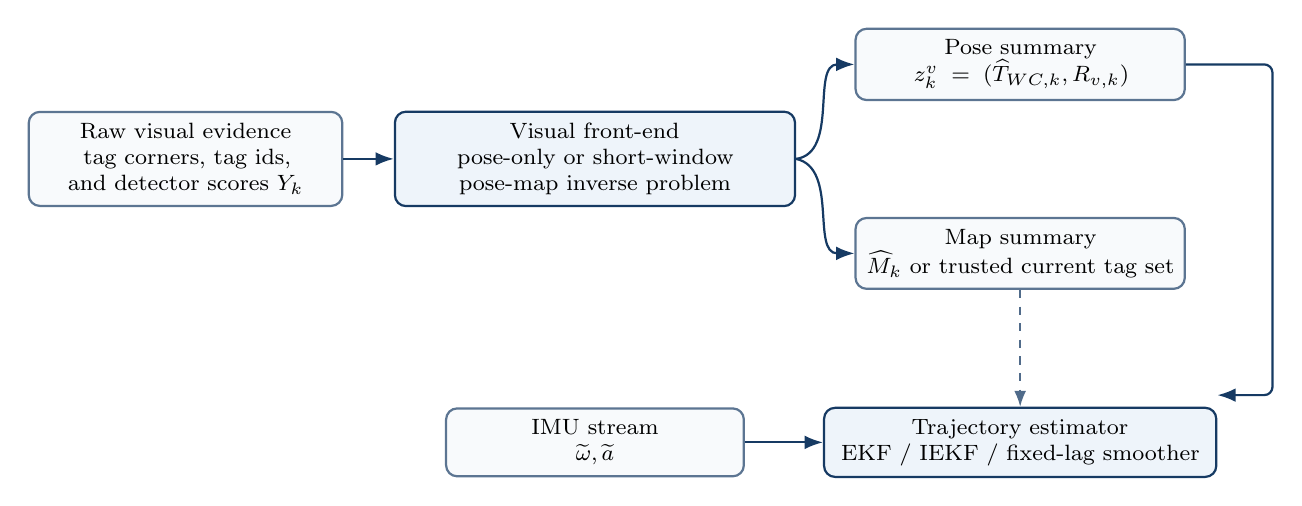
\begin{tikzpicture}[font=\footnotesize, >=Latex, x=1cm, y=1cm]
  \node[reportsoft, text width=3.7cm] (pixels) at (0,0) {Raw visual evidence\\tag corners, tag ids, and detector scores $Y_k$};
  \node[reportbox, text width=4.8cm] (front) at (5.2,0) {Visual front-end\\pose-only or short-window pose-map inverse problem};
  \node[reportsoft, text width=3.9cm] (pose) at (10.6,1.2) {Pose summary\\$z_k^v=(\widehat T_{WC,k},R_{v,k})$};
  \node[reportsoft, text width=3.9cm] (map) at (10.6,-1.2) {Map summary\\$\widehat M_k$ or trusted current tag set};
  \node[reportsoft, text width=3.5cm] (imu) at (5.2,-3.6) {IMU stream\\$\widetilde\omega,\widetilde a$};
  \node[reportbox, text width=4.7cm] (est) at (10.6,-3.6) {Trajectory estimator\\EKF / IEKF / fixed-lag smoother};
  \coordinate (poseouter) at ($(pose.east)+(1.1,0)$);
  \coordinate (poseentry) at ([yshift=6mm]est.east);
  \draw[reportarrow] (pixels) -- (front);
  \draw[reportarrow] (front.east) to[out=8,in=180] (pose.west);
  \draw[reportarrow] (front.east) to[out=-12,in=180] (map.west);
  \draw[reportarrow, rounded corners=3pt] (pose.east) -- (poseouter) -- (poseouter |- poseentry) -- (poseentry);
  \draw[reportdash] (map.south) -- (est.north);
  \draw[reportarrow] (imu) -- (est);
\end{tikzpicture}
\caption{Reduced visual interface. Raw pixels are consumed by a front-end inverse problem; the real-time estimator receives IMU data together with a pose summary and, when retained, a slowly updated tag-map summary.}
\end{figure}

\section{Inference structure: exact posterior and practical approximations}
\NotationTable{
$\Pi(d\bar x,dM,dc,db_{\mathrm{map}}\mid y^u,Y)$ & Full posterior measure on trajectory, map, and visual nuisance variables conditioned on raw IMU and raw visual data.\\
$\Pi_{\mathrm{ref}}$ & Product reference prior measure $\Pi_0\otimes\pi_M\otimes\Pi_c\otimes\pi_{\mathrm{map}}$.\\
$\widetilde\Pi(d\bar x,dc,db_{\mathrm{map}}\mid y^u,z^v,\widehat M)$ & Reduced approximate posterior after replacing raw pixels by front-end summaries.\\
$\Phi(\cdot)$ & Negative log likelihood or data-misfit functional.\\
$J(\cdot)$ & Discretized negative log posterior / MAP objective.\\
$\tilde f_k,\tilde g_k$ & Transition and pseudo-measurement kernels in the reduced sampled state-space model.}

At the fully Bayesian level there are four unknown objects: the continuous trajectory curve $\bar x(\cdot)$, the stationary auxiliary-tag map $M$, the temporally correlated visual-error process $c$, and the sequence-level visual bias $b_{\mathrm{map}}$. The clean posterior on these unknowns is a probability measure. If $y^u$ denotes the raw IMU stream and $Y$ the raw visual stream, then Bayes' formula is written symbolically as
\begin{equation}
\Pi(d\bar x,dM,dc,db_{\mathrm{map}}\mid y^u,Y)
\propto p(y^u\mid \bar x)\,p(Y\mid \bar x,M,c,b_{\mathrm{map}})\,\Pi_0(d\bar x)\,\pi_M(dM)\,\Pi_c(dc)\,\pi_{\mathrm{map}}(db_{\mathrm{map}}).
\label{eq:path_space_posterior_sweep}
\end{equation}
This is the most faithful statement of the inverse problem. It says: start from a prior law on trajectories and nuisance variables, then condition that law on the observed data. To make the Radon--Nikodym formula precise, introduce the product reference prior measure
\[
\Pi_{\mathrm{ref}}=\Pi_0\otimes\pi_M\otimes\Pi_c\otimes\pi_{\mathrm{map}}.
\]
Then one may write
\begin{equation}
\frac{d\Pi}{d\Pi_{\mathrm{ref}}}(\bar x,M,c,b_{\mathrm{map}})
\propto \exp\!\big(-\Phi_u(\bar x;y^u)-\Phi_v(\bar x,M,c,b_{\mathrm{map}};Y)\big).
\label{eq:rn_derivative_sweep}
\end{equation}
This notation emphasizes that the posterior is still a measure on functions, not yet a finite-dimensional Gaussian vector \citep{stuart2010inverse,hairer2007bayesian}.

In the reduced real-time formulation the raw visual data $Y$ are first converted into front-end outputs $(z^v,\widehat M)$, and the posterior is correspondingly replaced by the reduced model
\begin{equation}
\widetilde\Pi(d\bar x,dc,db_{\mathrm{map}}\mid y^u,z^v,\widehat M)
\propto p(y^u\mid \bar x)\,\tilde p(z^v\mid \bar x,\widehat M,c,b_{\mathrm{map}})\,\Pi_0(d\bar x)\,\Pi_c(dc)\,\pi_{\mathrm{map}}(db_{\mathrm{map}}).
\label{eq:reduced_path_space_posterior_sweep}
\end{equation}
Here $\tilde p$ is a pseudo-likelihood induced by the front-end condensation of the image data; it is not the raw pixel likelihood itself. Equation~\eqref{eq:reduced_path_space_posterior_sweep} is therefore an approximate reduced model, and it is this reduced model that the online filter approximates later in the report.

\subsection{Three numerical routes from the posterior to an estimator}
\NotationTable{
MCMC / SMC & Sampling-based approximation of the posterior law.\\
MAP & Maximum a posteriori estimate obtained by minimizing the negative log posterior.\\
Fixed lag & Sliding-window approximation that repeatedly solves a recent MAP problem.\\
EKF / IEKF & Recursive Gaussian approximation to the filtering posterior.}

There are three standard ways to turn the Bayesian inverse problem into a numerical algorithm.

\textbf{Route A: sample the posterior.} One can approximate the full posterior in \eqref{eq:path_space_posterior_sweep} by Markov-chain Monte Carlo or by sequential Monte Carlo. This is closest to the mathematically exact Bayesian formulation and best reflects multimodality or non-Gaussian uncertainty, but it is usually too expensive for 60~Hz online pose tracking.

\textbf{Route B: compute a MAP estimate.} After choosing a finite-dimensional discretization and local coordinates, one obtains a cost functional of the form
\begin{equation}
J(X,M,c,b_{\mathrm{map}})=\Phi_u(X;U)+\Phi_v(X,M,c,b_{\mathrm{map}};Y)+J_{\mathrm{prior}}(X,M,c,b_{\mathrm{map}}),
\end{equation}
and then solves
\begin{equation}
(X^\star,M^\star,c^\star,b_{\mathrm{map}}^\star)=\argmin J.
\end{equation}
Here $J_{\mathrm{prior}}$ collects the negative log prior terms in the chosen local coordinates. This becomes the factor-graph / bundle-adjustment view used by fixed-lag smoothers and modern VIO systems \citep{leutenegger2015okvis,forster2017preintegration,kaess2012isam2}. Figure~\ref{fig:factor_graph_joint_problem} should be read as the sparsity pattern of that exact joint MAP problem after discretizing the trajectory: blue nodes are unknown body states, green nodes are static tag poses, orange boxes are residual factors, and an edge means that residual term depends on that variable. It is therefore a coupling graph, not a process-flow diagram.

\begin{figure}[t]
\centering
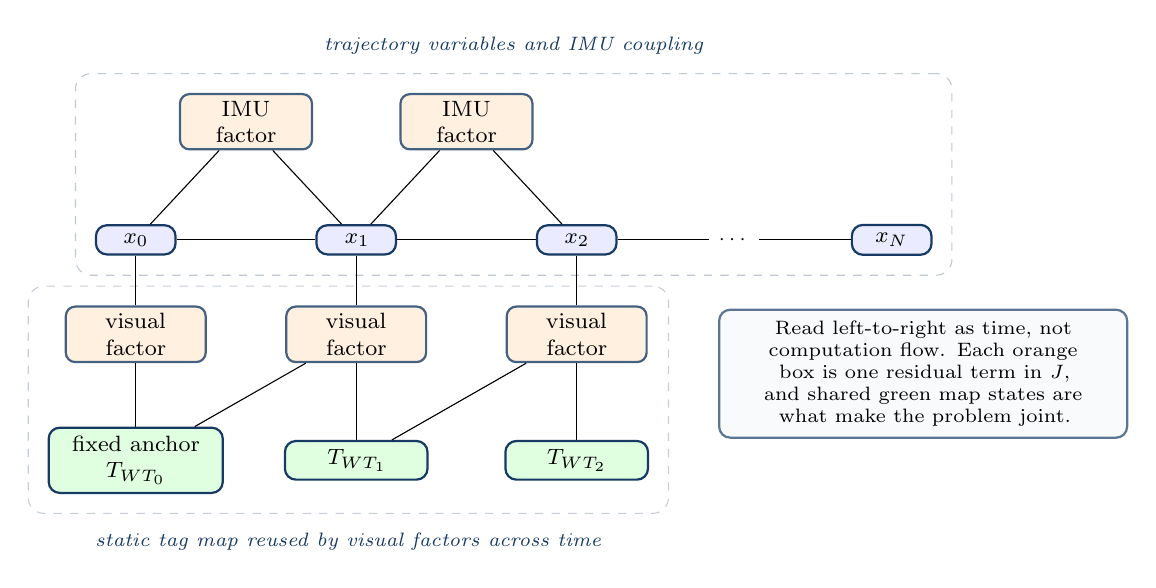
\begin{tikzpicture}[font=\footnotesize, >=Latex, x=1cm, y=1cm]
  \node[reportstate, text width=0.8cm] (x0) at (0,0.2) {$x_0$};
  \node[reportstate, text width=0.8cm] (x1) at (2.8,0.2) {$x_1$};
  \node[reportstate, text width=0.8cm] (x2) at (5.6,0.2) {$x_2$};
  \node[font=\scriptsize] (dots) at (7.6,0.2) {$\cdots$};
  \node[reportstate, text width=0.8cm] (xN) at (9.6,0.2) {$x_N$};
  \node[reportfactor, text width=1.5cm] (u01) at (1.4,1.7) {IMU\\factor};
  \node[reportfactor, text width=1.5cm] (u12) at (4.2,1.7) {IMU\\factor};
  \node[reportfactor, text width=1.6cm] (v0) at (0,-1.0) {visual\\factor};
  \node[reportfactor, text width=1.6cm] (v1) at (2.8,-1.0) {visual\\factor};
  \node[reportfactor, text width=1.6cm] (v2) at (5.6,-1.0) {visual\\factor};
  \node[reportmap, text width=2.0cm] (anchor) at (0,-2.6) {fixed anchor\\$T_{WT_0}$};
  \node[reportmap, text width=1.6cm] (m1) at (2.8,-2.6) {$T_{WT_1}$};
  \node[reportmap, text width=1.6cm] (m2) at (5.6,-2.6) {$T_{WT_2}$};
  \node[draw=Accent!28, dashed, rounded corners=2mm, inner sep=7pt, fit=(x0)(xN)(u01)(u12)] (trajgrp) {};
  \node[draw=Accent!25, dashed, rounded corners=2mm, inner sep=7pt, fit=(anchor)(m2)(v0)(v2)] (mapgrp) {};
  \node[font=\scriptsize\itshape, text=Accent] at ($(trajgrp.north)+(0,0.35)$) {trajectory variables and IMU coupling};
  \node[font=\scriptsize\itshape, text=Accent] at ($(mapgrp.south)+(0,-0.35)$) {static tag map reused by visual factors across time};
  \node[reportsoft, text width=4.9cm, font=\scriptsize] (note) at (10.0,-1.5) {Read left-to-right as time, not computation flow. Each orange box is one residual term in $J$, and shared green map states are what make the problem joint.};
  \draw (x0) -- (x1) -- (x2) -- (dots) -- (xN);
  \draw (u01) -- (x0);
  \draw (u01) -- (x1);
  \draw (u12) -- (x1);
  \draw (u12) -- (x2);
  \draw (anchor) -- (v0) -- (x0);
  \draw (anchor) -- (v1);
  \draw (m1) -- (v1) -- (x1);
  \draw (m1) -- (v2);
  \draw (m2) -- (v2) -- (x2);
\end{tikzpicture}
\caption{Sparsity pattern of the exact joint MAP problem. Body states $x_k$ and static tag poses $T_{WT_j}$ are optimized together; IMU factors couple consecutive states, while visual factors couple each frame state to the anchor or auxiliary tags visible in that frame. The visual-correlation variables $c$ and $b_{\mathrm{map}}$ are omitted for readability.}
\label{fig:factor_graph_joint_problem}
\end{figure}

The key structural point is the repeated reuse of the same static tag variables. The auxiliary-tag states $T_{WT_1},T_{WT_2},\ldots$ connect to visual factors from multiple frames, so the exact posterior is genuinely joint over trajectory and map. A two-stage front-end/back-end decomposition later in the report is therefore a deliberate approximation to this graph, not the graph itself.

\textbf{Route C: approximate the filtering posterior recursively by a Gaussian.} One computes only the sequence of filtering posteriors of the reduced Markov state
\begin{equation}
p(s_k\mid \mathcal D_{0:k},\widehat M),
\end{equation}
replacing each by a Gaussian in local coordinates around a nominal state. This yields EKF, IEKF, or related recursive filters \citep{mourikis2007msckf,barrau2017invariant,sarkka2023bayesian}.

\subsection{From the continuous posterior to the discrete Bayesian recursion}
\NotationTable{
$t_k$ & Sample times, typically camera frame times.\\
$\mathcal U_k$ & IMU packets collected between $t_k$ and $t_{k+1}$.\\
$s_k$ & Markov state used by the reduced state-space model, typically $s_k=(x_k,c_k,b_{\mathrm{map}})$.\\
$\tilde f_k(s_{k+1}\mid s_k)$ & Discrete transition kernel induced by inertial dynamics and any retained nuisance-state dynamics.\\
$\tilde g_k(z_k^v\mid s_k;\widehat M)$ & Pseudo-measurement kernel induced by the front-end summary at time $k$.}

To obtain an online estimator, sample the path at times $t_0,\dots,t_N$ and build a finite-dimensional Markov state. The extended sampled prior from \eqref{eq:markov_factorization_from_curve} is Markov on $\tilde x_k=(R_k,p_k,v_k,\omega_k,b_{g,k},b_{a,k})$. Practical filters usually condition on the IMU packets and retain the reduced body state
\begin{equation}
x_k=(R_k,p_k,v_k,b_{g,k},b_{a,k}).
\end{equation}
If the colored visual error $c_k$ and the static bias $b_{\mathrm{map}}$ are estimated explicitly, define
\begin{equation}
s_k=(x_k,c_k,b_{\mathrm{map}});
\end{equation}
otherwise they are omitted from $s_k$ and absorbed into an inflated visual-noise model. The reduced discrete posterior then takes the state-space form
\begin{align}
p(s_{0:N}\mid \mathcal D_{0:N},\widehat M)
&\propto p(s_0)
\prod_{k=0}^{N-1} \tilde f_k(s_{k+1}\mid s_k)
\prod_{k=0}^{N} \tilde g_k(z_k^v\mid s_k;\widehat M).
\label{eq:discrete_posterior_recursion_sweep}
\end{align}
The exact filtering recursion for this reduced state-space model is then
\begin{equation}
p(s_k\mid \mathcal D_{0:k},\widehat M)
\propto
\tilde g_k(z_k^v\mid s_k;\widehat M)
\int \tilde f_{k-1}(s_k\mid s_{k-1})\,p(s_{k-1}\mid \mathcal D_{0:k-1},\widehat M)\,ds_{k-1}.
\label{eq:exact_filtering_recursion_sweep}
\end{equation}
Everything that comes later---particle filters, MAP smoothers, EKF, IEKF---is an approximation either to this reduced recursion or, one level up, to the original raw-pixel posterior measure.

\subsection{How the Kalman filter is obtained as a simplification}
\NotationTable{
$\hat x_{k|k-1},P_{k|k-1}$ & Predicted mean and covariance of the filtered state before incorporating frame $k$.\\
$\hat x_{k|k},P_{k|k}$ & Updated mean and covariance after frame $k$.\\
$\delta s_k$ & Local error coordinates for the state actually linearized; in the baseline body-state filter $\delta s_k=\delta x_k$.\\
$F_k,G_k,H_k$ & Jacobians of the transition, noise injection, and measurement models.\\
$K_k,S_k$ & Kalman gain and innovation covariance.}

The Kalman filter is exact only for linear dynamics, linear measurements, and Gaussian noise in a vector space. Our problem violates all three conditions: the process and measurement models are nonlinear, and orientation / pose live on manifolds. The practical route to a Kalman-like algorithm is therefore:
\begin{enumerate}
  \item choose a discrete state $x_k$ sampled from the continuous curve;
  \item propagate a nominal state by the nonlinear inertial model;
  \item define a local Euclidean error state $\delta x_k$ in tangent coordinates;
  \item linearize the transition and measurement models around the current nominal state;
  \item approximate the local filtering posterior by a Gaussian in the error coordinates.
\end{enumerate}
This is the error-state EKF / IEKF construction.

For the present problem the nominal state is
\begin{equation}
\hat x_k=(\hat R_k,\hat p_k,\hat v_k,\hat b_{g,k},\hat b_{a,k}),
\end{equation}
and the baseline body-state error is
\begin{equation}
\delta x_k=\begin{bmatrix}
\delta\theta_k\\ \delta p_k\\ \delta v_k\\ \delta b_{g,k}\\ \delta b_{a,k}
\end{bmatrix}\in\R^{15}.
\label{eq:error_state_definition_sweep}
\end{equation}
If quaternions are used internally, $\delta\theta_k$ is \emph{still} 3-dimensional; only the stored nominal orientation changes from $\hat R_k$ to $\hat q_k$. If $c_k$ and/or $b_{\mathrm{map}}$ are estimated explicitly, then $\delta x_k$ is augmented by the corresponding Euclidean error coordinates.

The linearized prediction step is
\begin{equation}
\delta x_{k+1}=F_k\delta x_k+G_kn_k,
\qquad
P_{k+1|k}=F_kP_{k|k}F_k\tran+G_kQ_kG_k\tran.
\label{eq:ekf_prediction_sweep}
\end{equation}
The visual pseudo-measurement model is written on the pose manifold as
\begin{equation}
h_k(x_k,c_k,b_{\mathrm{map}})
=\Log\!\left(\widehat T_{WC,k}^{-1}T_{WB,k}T_{BC}\right)-b_{\mathrm{map}}-c_k.
\label{eq:visual_residual_filter_sweep}
\end{equation}
Around the predicted nominal state $\hat s_{k|k-1}$, this measurement function is linearized as
\begin{equation}
h_k(s_k)\approx h_k(\hat s_{k|k-1})+H_k\delta s_k+\nu_k,
\qquad
\nu_k\sim\mathcal N(0,R_{v,k}),
\end{equation}
where $\hat s_{k|k-1}$ denotes the predicted nominal state for whichever local state is being linearized, and $\delta s_k$ denotes either the 15-state body error or the augmented local error state. The corresponding innovation is
\begin{equation}
y_k^v=-h_k(\hat s_{k|k-1}),
\end{equation}
leading to the standard Kalman update
\begin{equation}
S_k=H_kP_{k|k-1}H_k\tran+R_{v,k},
\qquad
K_k=P_{k|k-1}H_k\tran S_k^{-1},
\end{equation}
\begin{equation}
\delta \hat s_{k|k}=K_ky_k^v,
\qquad
P_{k|k}=(I-K_kH_k)P_{k|k-1}(I-K_kH_k)\tran+K_kR_{v,k}K_k\tran.
\label{eq:joseph_update_sweep}
\end{equation}
Finally, the correction is injected back onto the manifold:
\begin{equation}
\hat R_{k|k}=\hat R_{k|k-1}\Exp([\delta\hat\theta_k]_{\times}),
\qquad
\hat p_{k|k}=\hat p_{k|k-1}+\delta\hat p_k,
\end{equation}
with analogous additive updates for velocity, biases, and any explicitly retained Euclidean nuisance states. In a quaternion implementation the rotational correction is written as
\begin{equation}
\hat q_{k|k}=\hat q_{k|k-1}\otimes \delta q_k,
\qquad
\delta q_k\approx\begin{bmatrix}1\\\Half\delta\hat\theta_k\end{bmatrix}.
\end{equation}
Thus the Kalman filter is not a different model from the Bayesian inverse problem. It is a tractable local-Gaussian approximation to the same posterior, obtained after discretization and linearization.

\subsection{When the Kalman simplification is appropriate and when it is not}
\NotationTable{
Unimodal posterior & A posterior well approximated by one Gaussian bump in local coordinates.\\
Linearization basin & Region in which the current nominal state is close enough to the true state for linearization to be accurate.\\
Reacquisition & First visual correction after a visual dropout interval.}

The EKF / IEKF approximation is appropriate when the posterior remains close to unimodal, the visual updates arrive frequently enough to keep inertial drift under control, and initialization starts inside the basin of attraction of the correct solution. It becomes weak when long visual dropouts allow inertial propagation to drift far from the truth, when the visual front-end becomes ambiguous or produces multimodal hypotheses, when outliers are not sufficiently gated, or when the visual covariance is badly misspecified. In such regimes a fixed-lag smoother or a more robust sampling-based approximation is safer. This is why the practical implementation hierarchy later in the note recommends starting with a filter and then moving to fixed-lag smoothing when relinearization or delayed correction becomes important.
\chapter{Practical Implementation}

\section{Parameter and noise guide: prior, likelihood, and tuning roles}
\NotationTable{
$m_0,P_0$ & Mean and covariance of the initial-state prior.\\
$Q_v,Q_\omega$ & Trajectory-smoothness spectral densities in the prior-on-curves.\\
$Q_{bg},Q_{ba}$ & Bias random-walk spectral densities in the prior.\\
$R_g,R_a$ & IMU likelihood covariance or equivalent noise-density parameters.\\
$R_{v,k}$ & Visual pose covariance at frame $k$.\\
$\sigma_q,\sigma_0,\alpha_A,\alpha_\theta,\alpha_b$ & Pixel-to-pose noise parameters used to build $R_{v,k}$.\\
$\rho_p,\rho_R,Q_c$ & Colored visual-noise hyperparameters for the latent process $c_k$.\\
$\Sigma_{\mathrm{map}}$ & Prior covariance of the sequence-level map / anchor bias term.}

A frequent source of confusion is mixing up \emph{prior parameters} and \emph{likelihood parameters}. The matrices $Q_v,Q_\omega,Q_{bg},Q_{ba}$ and the initial parameters $m_0,P_0$ define the prior law. They say what kinds of trajectories and bias evolutions are plausible \emph{before} the current measurements are assimilated. By contrast, $R_g,R_a$, and $R_{v,k}$ are likelihood parameters. They describe the spread of the observed measurements around the model-predicted values.

A helpful mental model is:
\begin{itemize}
  \item prior parameters regularize the \emph{unknown trajectory};
  \item likelihood parameters regularize the \emph{mismatch between data and model};
  \item nuisance-state priors, such as $Q_c$ or $\Sigma_{\mathrm{map}}$, sit in between and regularize latent error processes that explain persistent discrepancies.
\end{itemize}

In practice, parameter selection should proceed hierarchically.
\begin{enumerate}
  \item Estimate $R_g,R_a$ and their continuous-time equivalents from stationary IMU data, preferably through Allan deviation analysis. Kalibr's IMU model uses continuous-time white-noise and bias-random-walk parameters of exactly this form \citep{kalibr_noise}.\
  \item Estimate or model $R_{v,k}$ frame by frame from the pose front-end Hessian or from a parametric geometry-driven model such as \eqref{eq:pixel_sigma_model_sweep}.\
  \item Set $m_0$ from the first trustworthy visual pose and $P_0$ by inflating the front-end covariance to reflect unmodeled setup uncertainty.\
  \item Tune $Q_v,Q_\omega,Q_{bg},Q_{ba}$ so that innovation statistics are consistent: too small gives under-dispersed posteriors, too large gives noisy or drifting estimates.\
  \item If residual autocorrelation remains high on the visual side, introduce $c_k$ with parameters $(\rho_p,\rho_R,Q_c)$ rather than forcing independent noise to explain correlated errors.
\end{enumerate}

\section{Representative numeric regime for a phone-on-arm lab experiment}
\NotationTable{
$\Delta t_c$ & Camera frame interval.\\
$f_{\mathrm{imu}}$ & IMU sampling rate.\\
$s$ & Tag side length.\\
$z$ & Camera-to-anchor range.\\
$\sigma_g,\sigma_a,\sigma_{bg},\sigma_{ba}$ & IMU white-noise and bias-random-walk strengths.}

This section gives two kinds of numbers: \emph{hardware facts} drawn from cited sources, and \emph{engineering starting values} for the model parameters used in this chapter. The latter are recommendations, not immutable truths.

\begin{table}[t]
\centering
\scriptsize
\setlength{\tabcolsep}{3.8pt}
\begin{tabularx}{\textwidth}{p{0.22\textwidth}p{0.18\textwidth}X}
\toprule
\textbf{Quantity} & \textbf{Representative value} & \textbf{Rationale / source}\\
\midrule
Phone video rate & $60$ fps & Google's dedicated Pixel 9a specs page lists rear-camera 4K and 1080p recording at $30/60$ fps; taking the $60$ fps mode as the working regime gives $\Delta t_c\approx 16.7$ ms for this example \citep{pixel9a_specs}.\\
Phone main-camera FoV & about $82^{\circ}$ & Google's Pixel hardware tech-specs page lists an $82^{\circ}$ field of view for the Pixel 9a wide camera \citep{pixel9a_specs}.\\
Phone motion-sensor rate & $200$ Hz limit for \texttt{registerListener()} on Android 12+ apps without the high-rate permission & Android documents that, for apps targeting Android~12 (API level~31) or higher, \texttt{registerListener()} is rate-limited to $200$ Hz for the affected motion and position sensors unless the app declares \texttt{HIGH\_SAMPLING\_RATE\_SENSORS} \citep{android_sensors_overview}.\\
Research tabletop arm reach & about $0.855$ m & The Franka Research~3 product page lists an $855$ mm reach; this is a realistic scale for anchor-to-workspace geometry in a lab manipulation setup \citep{franka_fr3}.\\
Robot repeatability & $<\pm 0.1$ mm & The official Franka Research~3 datasheet lists position repeatability below $\pm 0.1$ mm under ISO~9283 \citep{franka_fr3}.\\
Robot control rate & about $1$ kHz low-level control & Official FR3 materials describe $1$ kHz control and measurement access through the Franka Control Interface; this is much faster than $60$ Hz phone video and faster than the $200$ Hz Android sensor-rate limit without the high-rate permission \citep{franka_fr3,pixel9a_specs,android_sensors_overview}.\\
Practical tag sizes & $0.06$--$0.10$ m & Typical lab fiducials for arm-mounted phone experiments are in the 6--10 cm range; this is an engineering choice that keeps tags visible at about 0.4--1.2 m range.\\
Practical anchored range & $0.4$--$1.2$ m & Consistent with a tabletop arm of roughly 0.85 m reach plus camera offset and the need to keep the anchor visible at least at startup.\\
Example Kalibr \texttt{imu.yaml} values & $\sigma_a=1.86\times10^{-3}$ m/s$^2/\sqrt{\mathrm{Hz}}$, $\sigma_{ba}=4.33\times10^{-4}$ m/s$^3/\sqrt{\mathrm{Hz}}$, $\sigma_g=1.87\times10^{-4}$ rad/s$/\sqrt{\mathrm{Hz}}$, $\sigma_{bg}=2.66\times10^{-5}$ rad/s$^2/\sqrt{\mathrm{Hz}}$ & Kalibr's YAML-formats page shows these as example \texttt{imu.yaml} entries at an update rate of $200$ Hz; the units and continuous-time interpretation are documented separately in the Kalibr IMU-noise page, so these values are useful as a format-and-units example, not as a phone-specific default \citep{kalibr_yaml_example,kalibr_noise}.\\
\bottomrule
\end{tabularx}
\caption{Representative numbers for a phone-on-arm laboratory regime. Some are hardware facts from official specs; others are engineering starting points for model design or sanity-check performance levels.}
\end{table}

For a first implementation aimed at a robot arm moving in a lab around an anchored tag, a very reasonable working regime is:
\begin{itemize}
  \item camera at $60$ Hz,
  \item IMU at $100$--$200$ Hz,
  \item tag size $s\in[0.06,0.10]$ m,
  \item anchor range $z\in[0.4,1.2]$ m,
  \item path spans on the order of $0.1$--$0.5$ m in translation over the sequence,
  \item translational speeds on the order of $0.05$--$0.5$ m/s for careful tabletop motions,
  \item angular rates on the order of $5^{\circ}$/s to $60^{\circ}$/s for ordinary camera reorientation.
\end{itemize}
These last values are engineering design targets rather than universal physical constants; they simply place the prior and likelihood parameters in the right numerical regime for a lab arm rather than a UAV or car.



\section{Implementation architecture for the anchored multi-tag problem}
\NotationTable{
$M_k=\{(\widehat T_{WT_j,k},P_{m_j,k})\}_{j\in\mathcal J_k}$ & Current map manager state: a set of auxiliary-tag pose posteriors carried up to frame $k$.\\
$P_{m_j,k}\in\R^{6\times 6}$ & Local covariance of tag $j$ in tangent coordinates around $\widehat T_{WT_j,k}\in\SE$.\\
$\mathcal J_k$ & Set of auxiliary tags that have already been initialized by frame $k$.\\
$\mathcal V_k^{\mathrm{old}},\mathcal V_k^{\mathrm{new}}$ & Visible tags at frame $k$ that are already in the map, and visible tags observed for the first time.\\
$z_k^v=(\widehat T_{WC,k},R_{v,k})$ & Visual pose pseudo-measurement returned by the front-end in the staggered architecture.\\
$q_k(M)$ & Approximate recursive posterior carried for the static tag map in the staggered architecture.}

The previous chapter established the reference posterior and the reduced real-time interface built from visual front-end summaries. This section translates those objects into an implementation architecture. The central design choice is straightforward.
\begin{itemize}
    \item If accuracy and statistical correctness are the highest priorities, solve a \emph{joint} posterior over trajectory and static tag map.
    \item If online speed and modularity are the highest priorities, solve a \emph{staggered} approximation, but do so knowingly and record where correlations are being neglected.
\end{itemize}
The rest of the section explains how that architectural choice affects initialization, new-tag birth, reappearance handling, and map bookkeeping. Figure~\ref{fig:implementation_architecture_report} should be read as an engineering module diagram for the staggered approximation, not as a posterior graph like Figure~\ref{fig:factor_graph_joint_problem}. Solid arrows denote within-cycle information flow at frame $k$, while the dashed return path denotes persistent map information carried between cycles and reused by later localizations.

\begin{figure}[t]
\centering
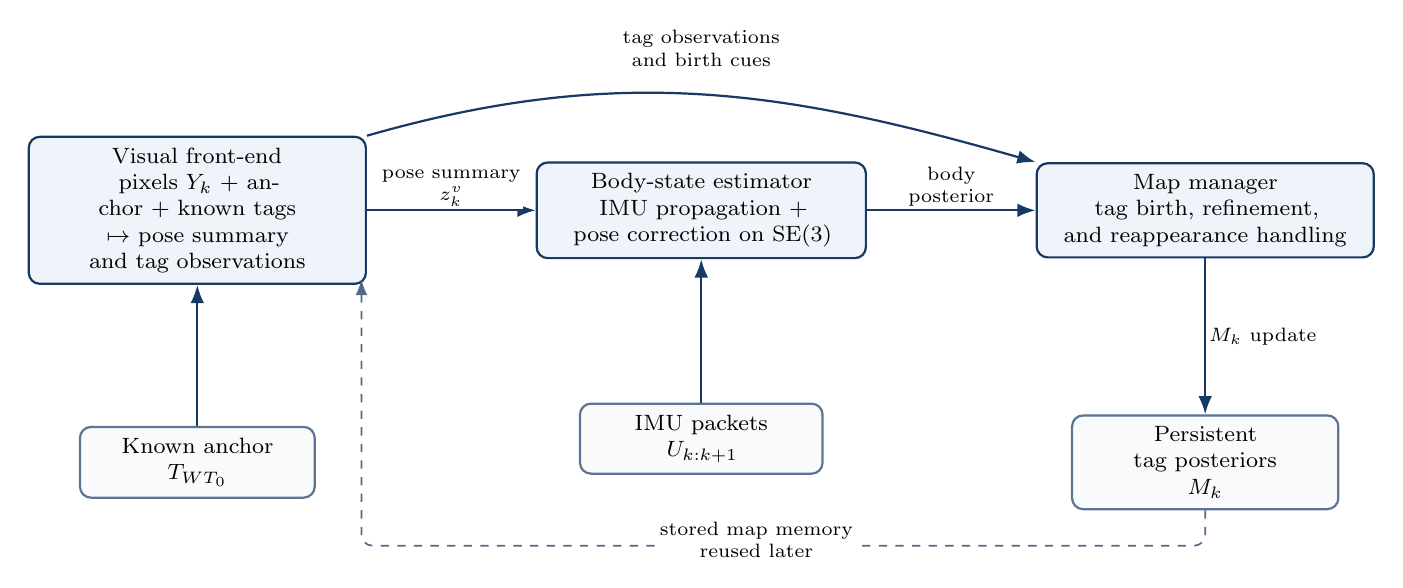
\begin{tikzpicture}[font=\footnotesize, >=Latex, x=1cm, y=1cm]
  \node[reportbox, text width=4.0cm] (front) at (0,0) {Visual front-end\\pixels $Y_k$ + anchor + known tags\\$\mapsto$ pose summary and tag observations};
  \node[reportbox, text width=3.9cm] (body) at (6.4,0) {Body-state estimator\\IMU propagation +\\pose correction on $\SE$};
  \node[reportbox, text width=4.0cm] (map) at (12.8,0) {Map manager\\tag birth, refinement,\\and reappearance handling};
  \node[reportsoft, text width=2.7cm] (anchor) at (0,-3.2) {Known anchor\\$T_{WT_0}$};
  \node[reportsoft, text width=2.8cm] (imu) at (6.4,-2.9) {IMU packets\\$U_{k:k+1}$};
  \node[reportsoft, text width=3.1cm] (tags) at (12.8,-3.2) {Persistent tag posteriors\\$M_k$};
  \draw[reportarrow] (anchor.north) -- (front.south);
  \draw[reportarrow] (imu.north) -- (body.south);
  \draw[reportarrow] (front.east) -- node[above, font=\scriptsize, fill=white, inner sep=1pt, align=center] {pose summary\\$z_k^v$} (body.west);
  \draw[reportarrow] (body.east) -- node[above, font=\scriptsize, fill=white, inner sep=1pt, align=center] {body\\posterior} (map.west);
  \draw[reportarrow] (front.north east) to[out=16,in=164] node[midway, above=9pt, font=\scriptsize, fill=white, inner sep=1pt, align=center] {tag observations\\and birth cues} (map.north west);
  \draw[reportarrow] (map) -- node[right, font=\scriptsize, fill=white, inner sep=1pt] {$M_k$ update} (tags);
  \draw[reportdash, rounded corners=4pt] (tags.south) -- ++(0,-0.45) -| ([xshift=-2pt,yshift=2pt]front.south east);
  \node[font=\scriptsize, fill=white, inner sep=1pt, align=center] at (7.1,-4.18) {stored map memory\\reused later};
\end{tikzpicture}
\caption{Staggered implementation architecture. The front-end uses current pixels together with the anchor and previously stored tag posteriors to produce a pose summary and tag observations; the body-state estimator fuses IMU packets with the pose summary; the map manager updates persistent auxiliary-tag posteriors using both the updated body posterior and visual tag information.}
\label{fig:implementation_architecture_report}
\end{figure}

\subsection{The exact joint solution}
The most defensible solution is to keep the entire unknown in one posterior. In discrete time this means solving for
\[
X_{0:N}=\{x_0,\ldots,x_N\},\qquad M=\{T_{WT_j}\}_{j\in\mathcal J_{\mathrm{aux}}},
\]
with posterior density
\[
p(X_{0:N},M\mid U_{0:N-1},Y_{0:N})
\propto
p_0(x_0)p_0(M)
\prod_{k=0}^{N-1} p(x_{k+1}\mid x_k,U_{k:k+1})
\prod_{k=0}^{N} p(Y_k\mid x_k,M).
\]
No information is used twice: each IMU packet contributes once through the process factor, each corner pixel contributes once through the camera model, and the static map and trajectory are inferred together. In practice this posterior is solved either by fixed-lag smoothing, batch MAP estimation, or posterior sampling as discussed earlier.

The fully joint method is especially attractive when
\begin{itemize}
    \item anchor visibility is intermittent,
    \item the auxiliary tags are numerous enough to act as a map,
    \item one wants statistically honest uncertainty on both camera pose and tag pose,
    \item and the same data must later support a trajectory posterior, a map posterior, and control diagnostics.
\end{itemize}
The price is computation and implementation complexity. A real-time version is usually built as a fixed-lag smoother, an EKF-SLAM style filter, or an incremental factor-graph system with a bounded set of actively tracked tags \citep{mourikis2007msckf,leutenegger2015okvis,forster2017preintegration,TagSLAM2019}.

\subsection{The speed-friendly staggered approximation}
The speed-friendly alternative is to separate the problem into three coupled but simpler pieces:
\begin{enumerate}
    \item a recursive body-state filter driven by IMU prediction,
    \item a visual front-end that uses the current map belief and the current pixels to produce a camera-pose posterior or pseudo-measurement,
    \item a tag-map manager that updates the posteriors of all stationary auxiliary tags using the current body posterior and current or delayed visual information.
\end{enumerate}
The staggered recursion is
\begin{align}
p^-(x_{k+1}) &= \int p(x_{k+1}\mid x_k,U_{k:k+1})\,p(x_k\mid \mathcal D_{0:k})\,dx_k,\\
q(z^v_{k+1}) &\approx q\bigl(T_{WC,k+1}\mid Y_{k+1},q_k(M),p^-(x_{k+1})\bigr),\\
p(x_{k+1}\mid \mathcal D_{0:k+1}) &\propto p(z^v_{k+1}\mid x_{k+1})\,p^-(x_{k+1}),\\
q_{k+1}(M) &\approx \mathcal U_M\bigl(q_k(M),Y_{k+1},p(x_{k+1}\mid \mathcal D_{0:k+1})\bigr),
\end{align}
where $\mathcal U_M$ denotes the chosen map-update mechanism.

This is only approximately Bayesian for two reasons. First, the same frame contributes both to the camera posterior and to the map posterior, creating camera--map correlation that is not fully retained unless one keeps the full joint covariance. Second, if the front-end itself used IMU information and the back-end then uses the same IMU packets again, the inertial information is double counted. Therefore a clean staggered design should obey the following rules.
\begin{itemize}
    \item The visual front-end should be \emph{visual only} when the back-end uses the IMU.
    \item The same frame's pixels should not be used twice as if they were independent: either they produce a pose pseudo-measurement \emph{or} they drive a joint state/map update, or one of the two uses is explicitly recognized as approximate.
    \item Newly seen tags should be initialized only after the camera/body posterior for the current frame is already anchored and trustworthy.
    \item Freshly refined map information should not be recycled back into the same frame's camera update; in a separated architecture it should influence the next frame onward.
    \item Any map update that reuses the current frame's data should be interpreted as an assumed-density approximation, not as the exact posterior.
\end{itemize}
When these caveats are stated clearly, the staggered approximation is a defensible engineering choice and often the fastest route to a robust implementation.

\begin{figure}[t]
\centering
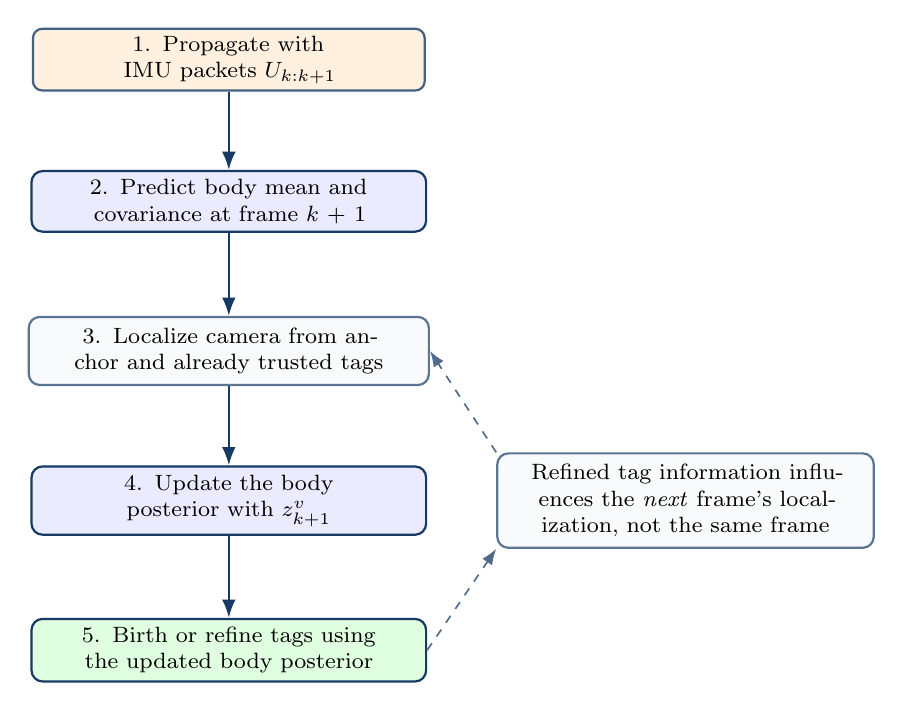
\begin{tikzpicture}[font=\footnotesize, >=Latex, x=1cm, y=1cm]
  \node[reportfactor, text width=4.8cm] (imu) at (0,0) {1. Propagate with IMU packets $U_{k:k+1}$};
  \node[reportstate, text width=4.8cm] (pred) at (0,-1.8) {2. Predict body mean and covariance at frame $k+1$};
  \node[reportsoft, text width=4.8cm] (cam) at (0,-3.7) {3. Localize camera from anchor and already trusted tags};
  \node[reportstate, text width=4.8cm] (body) at (0,-5.6) {4. Update the body posterior with $z_{k+1}^v$};
  \node[reportmap, text width=4.8cm] (map) at (0,-7.5) {5. Birth or refine tags using the updated body posterior};
  \node[reportsoft, text width=4.5cm] (next) at (5.8,-5.6) {Refined tag information influences the \emph{next} frame's localization, not the same frame};
  \draw[reportarrow] (imu) -- (pred);
  \draw[reportarrow] (pred) -- (cam);
  \draw[reportarrow] (cam) -- (body);
  \draw[reportarrow] (body) -- (map);
  \draw[reportdash] (map.east) -- (next.south west);
  \draw[reportdash] (next.north west) -- (cam.east);
\end{tikzpicture}
\caption{Update order in the staggered approximation. Camera localization uses only information available before the current tag-refinement step; fresh map updates are carried forward to the next frame.}
\label{fig:staggered_flow_report}
\end{figure}

\subsection{First frame: anchor guaranteed visible}
At frame $k=0$ the anchor is assumed visible. This makes initialization much simpler because the global gauge is fixed immediately.

\textbf{Step 1: initialize the camera pose from the anchor.} Solve the visual inverse problem using the anchor tag alone, or the anchor plus any already-known tags if such a map exists, to obtain
\[
q(T_{WC,0})\approx \Normal_{\seLie}(\widehat T_{WC,0},R_{v,0}).
\]
Then convert to body pose using the known camera--IMU extrinsic,
\[
\widehat T_{WB,0}=\widehat T_{WC,0}T_{CB},
\]
and propagate covariance through the local linearization.

\textbf{Step 2: initialize non-pose Euclidean components.} Choose
\[
v_{WB,0}\sim \Normal(0,P_{v0}),\qquad b_{g,0}\sim \Normal(0,P_{bg0}),\qquad b_{a,0}\sim \Normal(0,P_{ba0}),
\]
with conservative spreads unless a stationary segment is available.

\textbf{Step 3: initialize every auxiliary tag that is already visible.} For each $j\in\mathcal V_0\setminus\{0\}$, condition on the current camera posterior and solve a tag-pose inverse problem
\begin{equation}
\widehat T_{WT_j,0}
= \argmin_{T\in\SE}
\sum_{i=1}^{4}
\Bigl\|
\widetilde u_{0,j,i}-\pi\bigl(K,\widehat T_{CW,0}T\bar P_i^T\bigr)
\Bigr\|^2_{\Sigma_{0,j,i}^{-1}}.
\label{eq:tag_birth_conditional_init}
\end{equation}
Then initialize a broad covariance $P_{m_j,0}$ from the local Hessian, inflated to reflect uncertainty in the camera pose used for conditioning. Intuitively, the anchor gives the first camera pose, and the first camera pose gives the first absolute estimate of every co-visible auxiliary tag.

\subsection{First sighting of a new tag at a later frame (tag birth)}
Suppose tag $j$ is seen for the first time at frame $k>0$. Then there are two legitimate routes.

\textbf{Joint route.} In a joint filter or smoother, augment the state with a new static variable $T_{WT_j}$ and update the enlarged posterior directly using the current pixels. This is the statistically clean route.

\textbf{Staggered route.} In the speed-friendly design, use the current body posterior as a conditional prior and create a new tag posterior
\begin{equation}
p(T_{WT_j}\mid Y_k^j,\mathcal D_{0:k})
\propto
\int p(Y_k^j\mid x_k,T_{WT_j})\,p(x_k\mid\mathcal D_{0:k})\,dx_k\;p_0(T_{WT_j}).
\label{eq:new_tag_birth_integral}
\end{equation}
This integral is usually approximated by conditioning on the current body mean or sigma points. A practical implementation is:
\begin{enumerate}
    \item wait until the current camera/body posterior is well constrained by the anchor or by already-mapped tags,
    \item solve \eqref{eq:tag_birth_conditional_init} at the current frame using the camera posterior mean,
    \item assign a broad covariance that includes both pixel uncertainty and the uncertainty in the current camera pose,
    \item mark the tag as ``provisional'' until it has been observed repeatedly.
\end{enumerate}
\textbf{Important edge case.} If the camera sees only entirely new unknown tags and no anchor or already-initialized tags, then those tags cannot yet be anchored absolutely in the world frame. In that case the correct action is \emph{not} to force an absolute initialization. One should defer birth until a frame where the camera itself is well localized in the anchored frame.

\subsection{Tag disappearance and later reappearance}
A stationary tag that disappears for several frames does not require a special dynamic model. Its pose remains static:
\[
T_{WT_j,k+1}=T_{WT_j,k},
\]
possibly with a very small artificial process noise added only for numerical conditioning. Therefore during absence one simply carries its posterior forward,
\[
q_{k+1}(T_{WT_j}) = q_k(T_{WT_j}),
\]
while recording bookkeeping such as last seen time, number of successful updates, and recent residual quality.

When the tag reappears, one treats the previous tag posterior as the prior and performs an ordinary measurement update. In the joint formulation, the pixels for that tag simply re-enter the global likelihood. In the staggered formulation, the current body posterior and previous tag posterior produce a predicted pixel distribution, which is then used for gating and update. Formally,
\begin{equation}
p(T_{WT_j}\mid Y_k^j,\mathcal D_{0:k})
\propto
p(Y_k^j\mid x_k,T_{WT_j})\,p(T_{WT_j}\mid\mathcal D_{0:k-1}),
\label{eq:reappearing_tag_update}
\end{equation}
with the current body posterior either conditioned on jointly or approximated by its mean/covariance.

For robust practice, reappearing tags should be accepted only after a consistency gate:
\begin{itemize}
    \item predicted-vs-observed corner residual below threshold,
    \item correct decoded tag id,
    \item plausible depth and viewing geometry,
    \item and, if available, Mahalanobis innovation below a chosen threshold.
\end{itemize}

\subsection{How to keep track of all tags in code}
A simple and effective representation is to store each auxiliary tag as a record
\[
m_j = (\widehat T_{WT_j},P_{m_j},n_j,\tau_j,\eta_j),
\]
where $n_j$ is observation count, $\tau_j$ is last-seen timestamp, and $\eta_j$ is a small quality bundle such as mean residual, provisional/confirmed flag, and recent visibility streak. The whole map manager state is then
\[
M_k=\{m_j\}_{j\in\mathcal J_k}.
\]
No global alignment other than the anchor is assumed: every tag carries its own arbitrary 6-DoF pose in the anchored world frame.

The camera pose itself is tracked in exactly the same geometric space as each tag pose, namely a pose on $\SE$ plus a covariance on the corresponding tangent space. The difference is semantic, not mathematical: the camera pose is dynamic and time indexed, while each auxiliary-tag pose is static and time invariant.

\subsection{A compact implementation recipe}
For readers who want an executable checklist, the following is a good starting point.
\begin{enumerate}
    \item \textbf{Frame 0.} Use anchor pixels to initialize $T_{WC,0}$, then initialize $T_{WB,0}$, velocity, and biases. Initialize all co-visible auxiliary tags as provisional static poses with broad covariance.
    \item \textbf{Between frames.} Propagate the body posterior using IMU packets only.
    \item \textbf{At frame $k+1$.} Detect tag corners and ids. Split them into already-known tags and new tags.
    \item \textbf{Visual localization.} Use the anchor and any trustworthy known auxiliary tags to produce either a direct joint pixel update or a visual pose pseudo-measurement $z_{k+1}^v$.
    \item \textbf{Body update.} Fuse the visual information with the predicted body posterior.
    \item \textbf{Map update.} Update already-known visible auxiliary tags using the current body posterior. Initialize newly observed tags only if the current body posterior is trustworthy in the anchored world frame.
    \item \textbf{Bookkeeping.} Increment counts, store residual statistics, mark tags as confirmed after enough successful reobservations, and keep absent tags unchanged until they reappear.
\end{enumerate}
This recipe keeps the module boundaries clean while making the approximation points explicit.

\section{Kalman realization, sampling, and approximation pitfalls}
\NotationTable{
$\pi(\cdot)$ & Generic posterior density.\\
$\theta$ & Collective variable used in sampling, e.g. a block of poses or tag states.\\
$\alpha(\theta,\theta')$ & Metropolis--Hastings acceptance probability for a proposal $\theta\to\theta'$.\\
$\mathcal N(m,P)$ & Euclidean Gaussian approximation used by EKF/IEKF or Laplace approximations.\\
$\NIS,\NEES$ & Innovation and state consistency statistics used to validate the Gaussian approximation.}

\subsection{How the Kalman filter emerges from the Bayesian problem}
The exact filtering recursion was written in \eqref{eq:exact_filtering_recursion_sweep}. A Kalman-style filter appears only after several simplifications:
\begin{enumerate}
    \item discretize the curve prior into a Markov transition law,
    \item represent the posterior by a local Gaussian in tangent coordinates,
    \item linearize the process and measurement operators,
    \item assume that the necessary marginal or conditional distributions are adequately captured by their first two moments.
\end{enumerate}
Then the dynamic body state uses prediction
\[
\bar x_{k+1}=f(\widehat x_k,U_{k:k+1}),\qquad
\bar P_{k+1}=F_k P_k F_k^{\top}+G_kQ_kG_k^{\top},
\]
and update
\[
K_{k+1}=\bar P_{k+1}H_{k+1}^{\top}(H_{k+1}\bar P_{k+1}H_{k+1}^{\top}+R_{k+1})^{-1},
\]
with local state correction applied by the manifold update rules introduced in Chapter~1. In a joint EKF-SLAM style system, the state also carries selected tag poses and their cross-covariances with the body state. In the speed-friendly architecture, the body filter and tag-map manager are separated, sacrificing some statistical exactness for simplicity and speed.

\subsection{Metropolis--Hastings sampling for posterior visualization}
For scientific understanding and posterior visualization, it is useful to sample not only trajectories but also tag poses. Let
\[
\theta=(X_{0:N},M)
\]
or, for a fixed-lag window, a smaller block such as recent poses, recent biases, and the currently visible tag poses. Given a proposal density $q(\theta'\mid\theta)$, the Metropolis--Hastings acceptance probability is
\begin{equation}
\alpha(\theta,\theta')=
\min\left\{1,
\frac{\pi(\theta')\,q(\theta\mid\theta')}{\pi(\theta)\,q(\theta'\mid\theta)}
\right\}.
\label{eq:mh_acceptance_report}
\end{equation}
A practical choice is blockwise proposals in local coordinates:
\begin{itemize}
    \item propose several consecutive body poses in $\se(3)$ coordinates,
    \item propose velocity and bias blocks additively in $\R^3$,
    \item propose one or more tag poses in $\se(3)$ coordinates.
\end{itemize}
This is not meant for real-time estimation at 60~Hz. Its purpose is diagnostic and pedagogical: it reveals multimodality, non-Gaussianity, and tag--trajectory coupling that a local EKF approximation may hide. For example, one can visualize posterior samples of a reappearing tag's pose, or posterior tubes of the camera trajectory during partial occlusion.

\subsection{What counts as a statistical or probabilistic crime?}
Several implementation shortcuts are acceptable approximations. Several others are genuine mistakes.
\begin{itemize}
    \item \textbf{Double counting IMU.} If IMU is used inside the front-end to form $z_k^v$ and then used again in the back-end process model, inertial information has been counted twice.
    \item \textbf{Using the same pixels twice as if independent.} If a frame's pixels are first condensed into a pose posterior and then the same pixels are also used again to update the same latent variables without accounting for dependence, posterior uncertainty becomes too small.
    \item \textbf{Birth of a new tag without an anchored camera posterior.} A tag seen in isolation cannot be assigned a trustworthy absolute world pose unless the camera pose in the anchored frame is already known.
    \item \textbf{Treating tag poses as Euclidean vectors.} Tag pose covariance must live in local coordinates on $\SE$, not in arbitrary matrix-entry coordinates.
    \item \textbf{Ignoring time correlation in visual pseudo-measurements.} If the front-end reuses similar geometry frame after frame, assuming independent $R_{v,k}$ may lead to overconfident trajectory estimates.
\end{itemize}
On the other hand, the following are usually acceptable first approximations:
\begin{itemize}
    \item using the current camera mean to initialize a new tag and inflating its covariance,
    \item updating the static tag map in a separate delayed module,
    \item using a fixed-lag smoother to repair the neglected correlations of the real-time front-end.
\end{itemize}

\subsection{Assessment: is the staggered scheme reasonable?}
Yes. The staggered scheme is a reasonable option provided it is described honestly. It is not the exact joint posterior described in Chapter~1, but it is a principled approximation of it. In many practical systems this is a practical trade-off: the front-end manages raw pixels and geometry, the back-end manages real-time propagation and correction, and a slower map-refinement layer repairs the parts of the posterior that the fast filter cannot represent exactly. This is close in spirit to many mature recursive, smoothing, and factor-graph estimation systems even when they are not written in exactly the same notation \citep{mourikis2007msckf,leutenegger2015okvis,forster2017preintegration,kaess2012isam2,TagSLAM2019}.

\section{Synthesis and literature position}
The reference problem is a posterior on a trajectory curve together with a static auxiliary-tag map in an anchored world frame. The prior is a law on that mixed object: smooth body motion, slowly drifting biases, and static but initially unknown tag poses. In the full joint model the IMU contributes the inertial data-misfit and the camera contributes the raw-pixel likelihood through the tag projection model. If one solves everything jointly, the result is a direct Bayesian estimator over both trajectory and map. If one instead chooses a speed-friendly decomposition, the corresponding reduced model replaces the raw-pixel likelihood by a front-end-induced pseudo-likelihood on $z_k^v$ and is defensible only if the front-end is visual only, the IMU is used exactly once, new tags are created only when the current anchored camera posterior is trustworthy, absent tags remain latent static variables, and same-frame camera-plus-tag refinement is treated as an approximation whose neglected correlations are later repaired by a smoother or broader covariance inflation. The practical message is therefore simple: exact Bayes is the reference model, and recursive or fixed-lag estimators are computational approximations to it.

\subsection{How the literature positions these choices}
The Bayesian inverse-problem perspective treats trajectory and map as latent variables inferred from sensor data and priors \citep{stuart2010inverse}. Recursive Bayesian filtering and smoothing provide the general algorithmic backbone \citep{sarkka2023bayesian}. In visual--inertial robotics, filtering families such as MSCKF keep a Gaussian posterior over the current state and selected pose history \citep{mourikis2007msckf}. Optimization families such as IMU-preintegrated MAP smoothing, OKVIS, and VINS-Mono instead solve nonlinear MAP problems over keyframes or sliding windows of recent states, sometimes with structureless visual factors rather than explicit landmark states \citep{Forster2015,forster2017preintegration,leutenegger2015okvis,VINSMono2017}. Fiducial-tag systems such as TagSLAM explicitly represent static tag poses and body poses together in a factor graph \citep{TagSLAM2019}. Continuous-time Bayesian approaches such as STEAM place priors directly on the space of trajectories and then condition on observations \citep{Barfoot2014,anderson2015gp}. The anchored multi-tag method developed in this report fits naturally in this landscape as either a joint fiducial visual--inertial SLAM estimator or a conservative two-stage approximation to it.

\clearpage
\appendix
\chapter{Prior samples for interpretation and sanity checking}

\NotationTable{
$\Delta t$ & Discrete time step used for sampling; here $\Delta t=\tfrac{1}{60}$ s.\\
$N$ & Number of discrete states; in the annex $N=241$ corresponding to a $4$ s horizon.\\
$a_k,\alpha_k$ & Sampled translational acceleration and angular-acceleration drives at step $k$.\\
$\omega_k$ & Latent body angular velocity used only to generate the pose process in this annex.\\
$\mathrm{rpy}_k$ & Roll--pitch--yaw angles extracted from $R_k$ only for visualization; they are \emph{not} the coordinates used by the filter.}

This annex does not introduce a new inferential model. It samples a simple discrete-time approximation to the extended trajectory prior from Chapter~1. The purpose is pedagogical: it is much easier to understand the role of the prior hyperparameters once one sees typical paths they generate. In particular, the sampler keeps the latent angular velocity $\omega_k$ explicit so that the orientation process can be generated directly. This matches the extended-state prior discussion in Chapter~1; it is not literally the same object as the reduced IMU-conditioned filter recursion used later for online estimation.

For the simulation we use the discrete generative scheme
\begin{align}
p_{k+1} &= p_k + v_k \Delta t + \tfrac12 a_k \Delta t^2,\\
v_{k+1} &= v_k + a_k \Delta t,\\
R_{k+1} &= R_k \Exp\!\big((\omega_k \Delta t)^\wedge\big),\\
\omega_{k+1} &= \omega_k + \alpha_k \Delta t,\\
b_{g,k+1} &= b_{g,k} + \eta^{bg}_k,\\
b_{a,k+1} &= b_{a,k} + \eta^{ba}_k,
\end{align}
with independent Gaussian drives
\begin{align}
a_k &\sim \mathcal N(0,\sigma_a^2 I_3),\qquad
\alpha_k \sim \mathcal N(0,\sigma_\alpha^2 I_3),\\
\eta^{bg}_k &\sim \mathcal N(0,\sigma_{bg,\mathrm{rw}}^2 I_3),\qquad
\eta^{ba}_k \sim \mathcal N(0,\sigma_{ba,\mathrm{rw}}^2 I_3).
\end{align}
The sampled state shown in the plots is the filter-style state
\[
x_k=(R_k,p_k,v_k,b_{g,k},b_{a,k}),
\]
while the auxiliary variable $\omega_k$ is used internally only to generate the orientation process. For display we convert $R_k$ into roll, pitch, and yaw angles. This is a visualization choice only: the actual filter should still represent rotational uncertainty in local Lie coordinates or in a quaternion plus 3D error state.

\section{Prior values used for the illustrative samples}

\begin{table}[H]
\centering
\small
\setlength{\tabcolsep}{5pt}
\begin{tabularx}{\textwidth}{p{0.33\textwidth}p{0.22\textwidth}X}
\toprule
\textbf{Quantity} & \textbf{Value} & \textbf{Role in the prior sampler}\\
\midrule
Time step $\Delta t$ & $1/60$ s & Matches the camera-frame discretization used throughout the report.\\
Horizon $T$ & $4$ s & Short lab-style motion segment.\\
$\sigma_{p0}$ & $(0.01,0.01,0.01)$ m & Initial position spread.\\
$\sigma_{v0}$ & $(0.03,0.03,0.03)$ m/s & Initial velocity spread.\\
$\sigma_{\mathrm{rpy},0}$ & $(2,2,3)^\circ$ & Initial orientation spread, shown in Euler angles only for display.\\
$\sigma_{\omega0}$ & $(4,4,5)^\circ$/s & Initial angular-velocity spread used to drive the pose process.\\
$\sigma_a$ & $0.10$ m/s$^2$ & Translational acceleration roughness.\\
$\sigma_\alpha$ & $6^\circ$/s$^2$ & Angular-acceleration roughness.\\
$\sigma_{bg,0}$ & $(0.20,0.20,0.20)^\circ$/s & Initial gyroscope-bias spread.\\
$\sigma_{ba,0}$ & $(0.03,0.03,0.03)$ m/s$^2$ & Initial accelerometer-bias spread.\\
$\sigma_{bg,\mathrm{rw}}$ & $0.005^\circ$/s per step & Gyroscope-bias random-walk step scale.\\
$\sigma_{ba,\mathrm{rw}}$ & $0.001$ m/s$^2$ per step & Accelerometer-bias random-walk step scale.\\
\bottomrule
\end{tabularx}
\caption{Illustrative prior values used for the annex sampler. These values are not claimed to be universal; they are chosen to produce motions in a realistic phone-on-arm laboratory regime, with translation excursions on the order of a few tenths of a meter and orientation excursions on the order of a few tens of degrees over the $4$ s horizon.}
\end{table}

The script used to generate the figures in this annex is stored alongside the report as \texttt{sample\_prior\_paths.py}, together with the JSON file \texttt{prior\_sample\_parameters.json}. The figures can therefore be regenerated whenever the assumed prior regime is adjusted.

\section{Three-dimensional prior samples}

Figure~\ref{fig:prior_paths_3d_annex} shows eight sampled translation paths. The curves begin near the origin because the initial position prior is tight, then fan out as the sampled accelerations accumulate. This picture is the translational part of the prior alone; it is \emph{not} a posterior trajectory and it is not conditioned on data.

\begin{figure}[H]
\centering
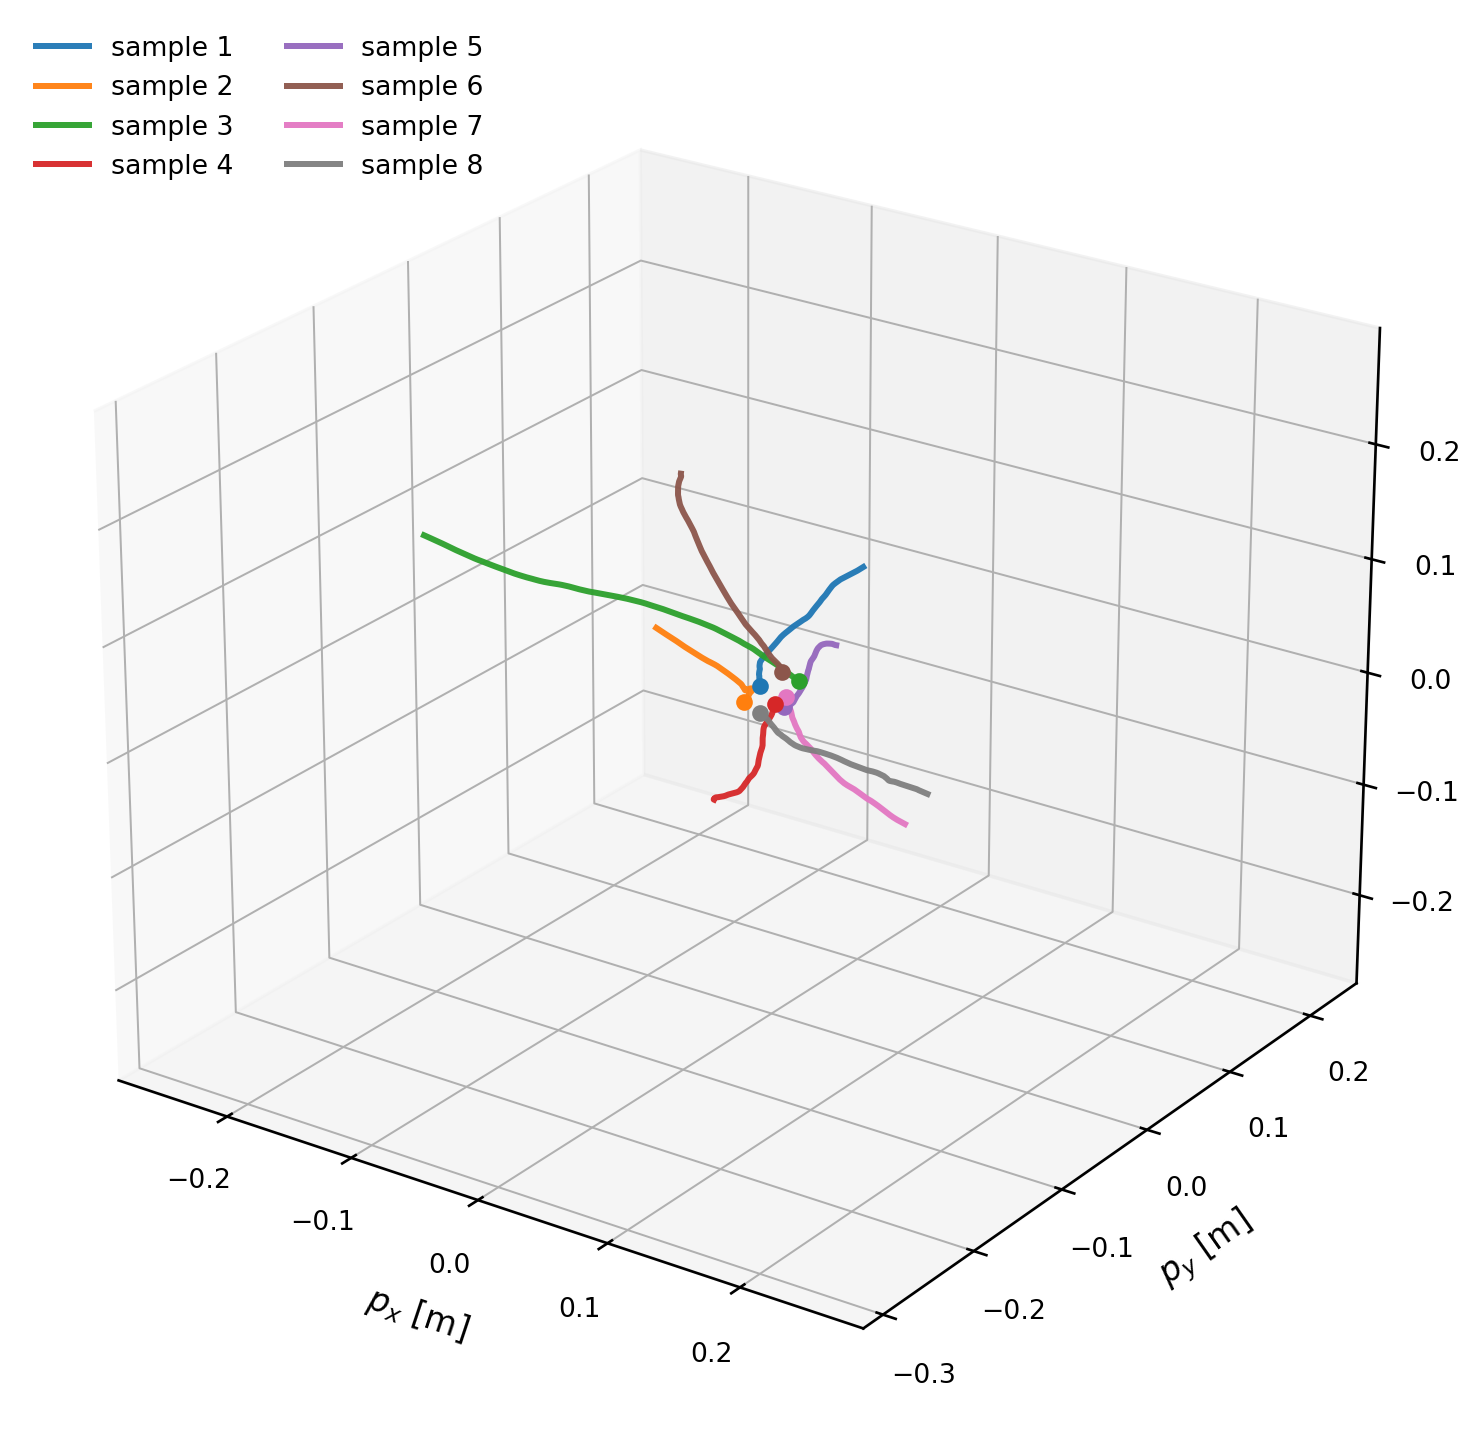
\includegraphics[width=0.92\textwidth]{prior_paths_3d.png}
\caption{Eight sample trajectories drawn from the discretized prior over a $4$ s interval at $60$ Hz. The paths illustrate the translational component of the prior before any measurement update is applied.}
\label{fig:prior_paths_3d_annex}
\end{figure}

To visualize that the prior actually lives on poses rather than on positions only, Figure~\ref{fig:prior_pose_glyphs_annex} overlays body-frame triads along one sample path. The translational path lies in $\R^3$, but the orientation evolves on $\SO(3)$ and is injected through the exponential-map update.

\begin{figure}[H]
\centering
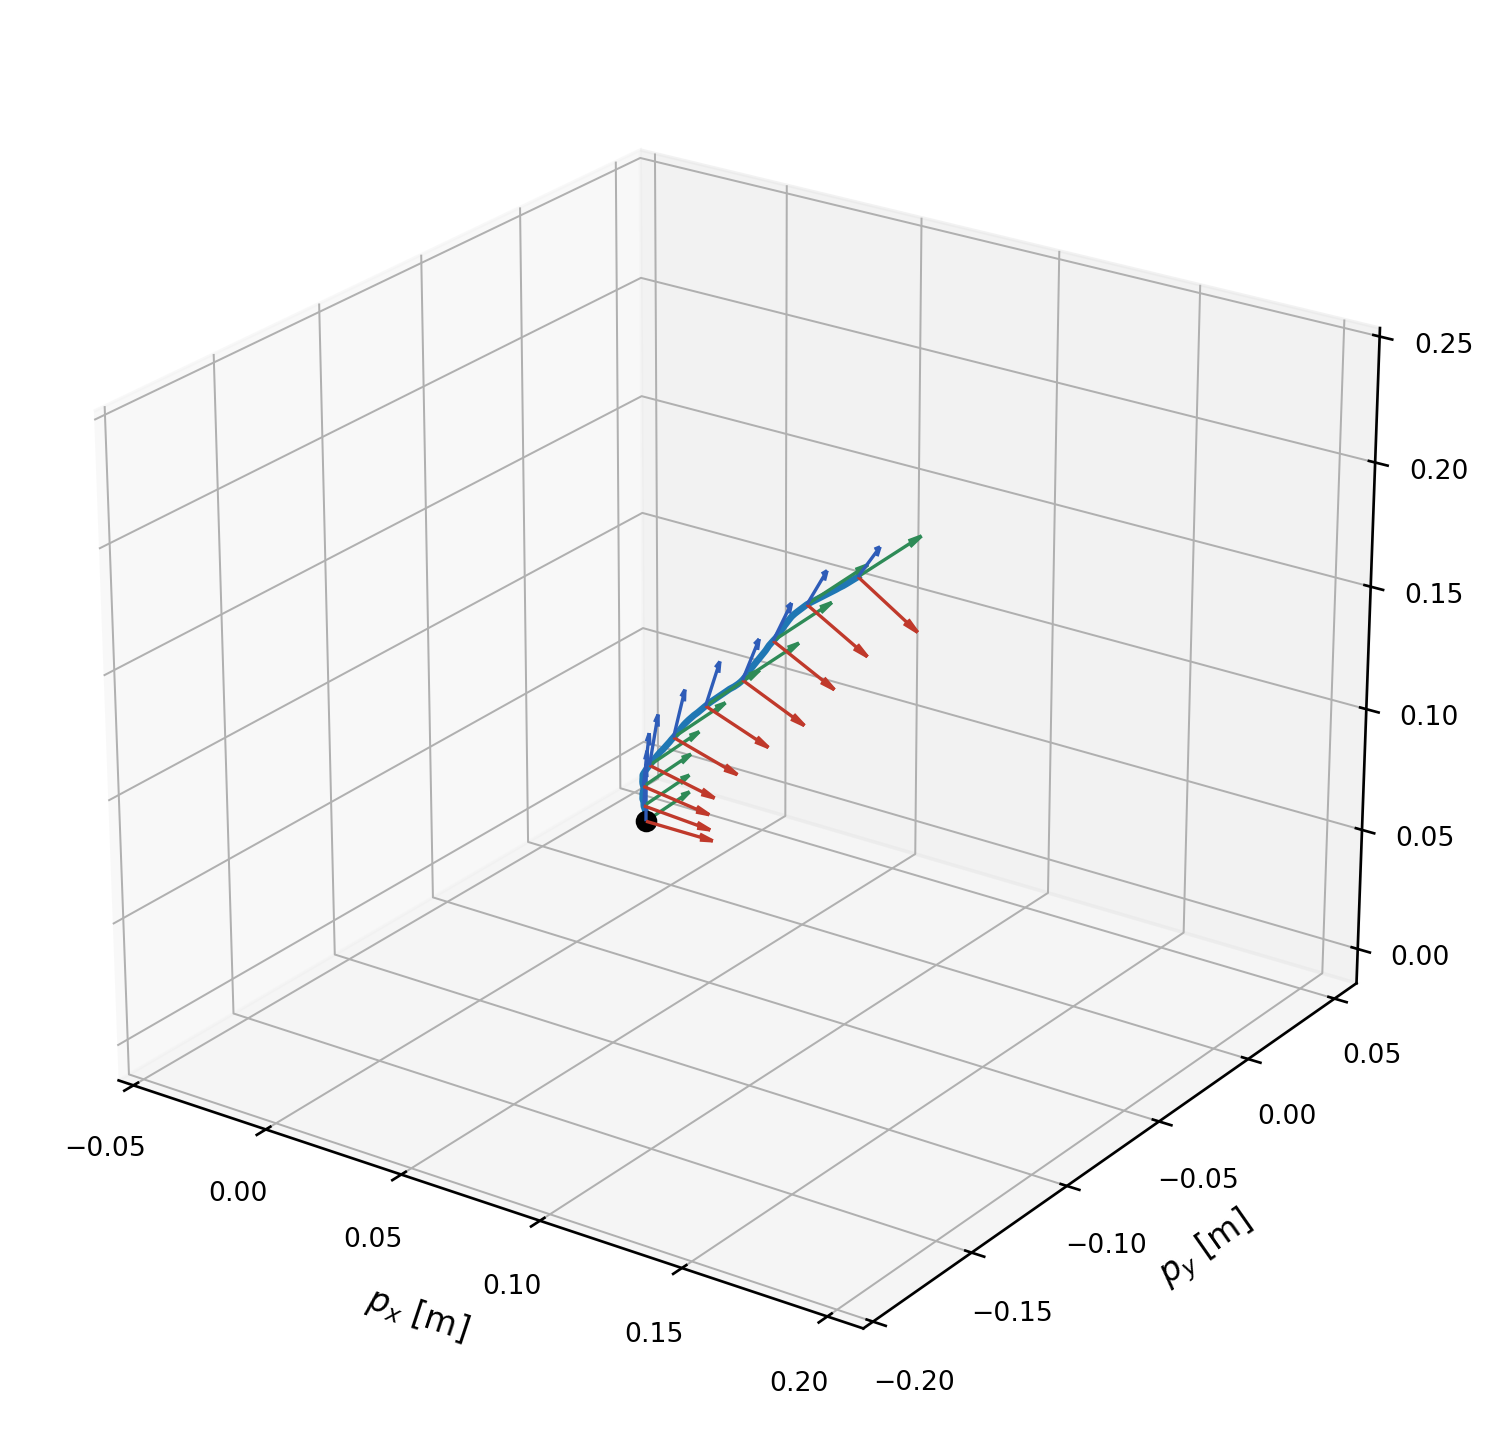
\includegraphics[width=0.92\textwidth]{prior_pose_glyphs.png}
\caption{One sampled pose trajectory with body-frame triads along the path. The translation is a path in $\R^3$, while the orientation component evolves on $\SO(3)$ and is updated multiplicatively.}
\label{fig:prior_pose_glyphs_annex}
\end{figure}

\section{State evolution of all filter variables}

Figure~\ref{fig:prior_state_entries_annex} shows the evolution of all entries of the filter-style state
\[
x_k=(R_k,p_k,v_k,b_{g,k},b_{a,k}).
\]
For readability, the orientation is displayed as roll, pitch, and yaw angles. The plots make the mixed geometry of the state visible: positions and velocities behave like ordinary Euclidean random walks with smoothness; the bias states evolve much more slowly; and the orientation display coordinates drift in a way that reflects accumulated angular velocity, even though the actual internal pose update is performed on the Lie group rather than by angle-wise addition.

\begin{figure}[p]
\centering
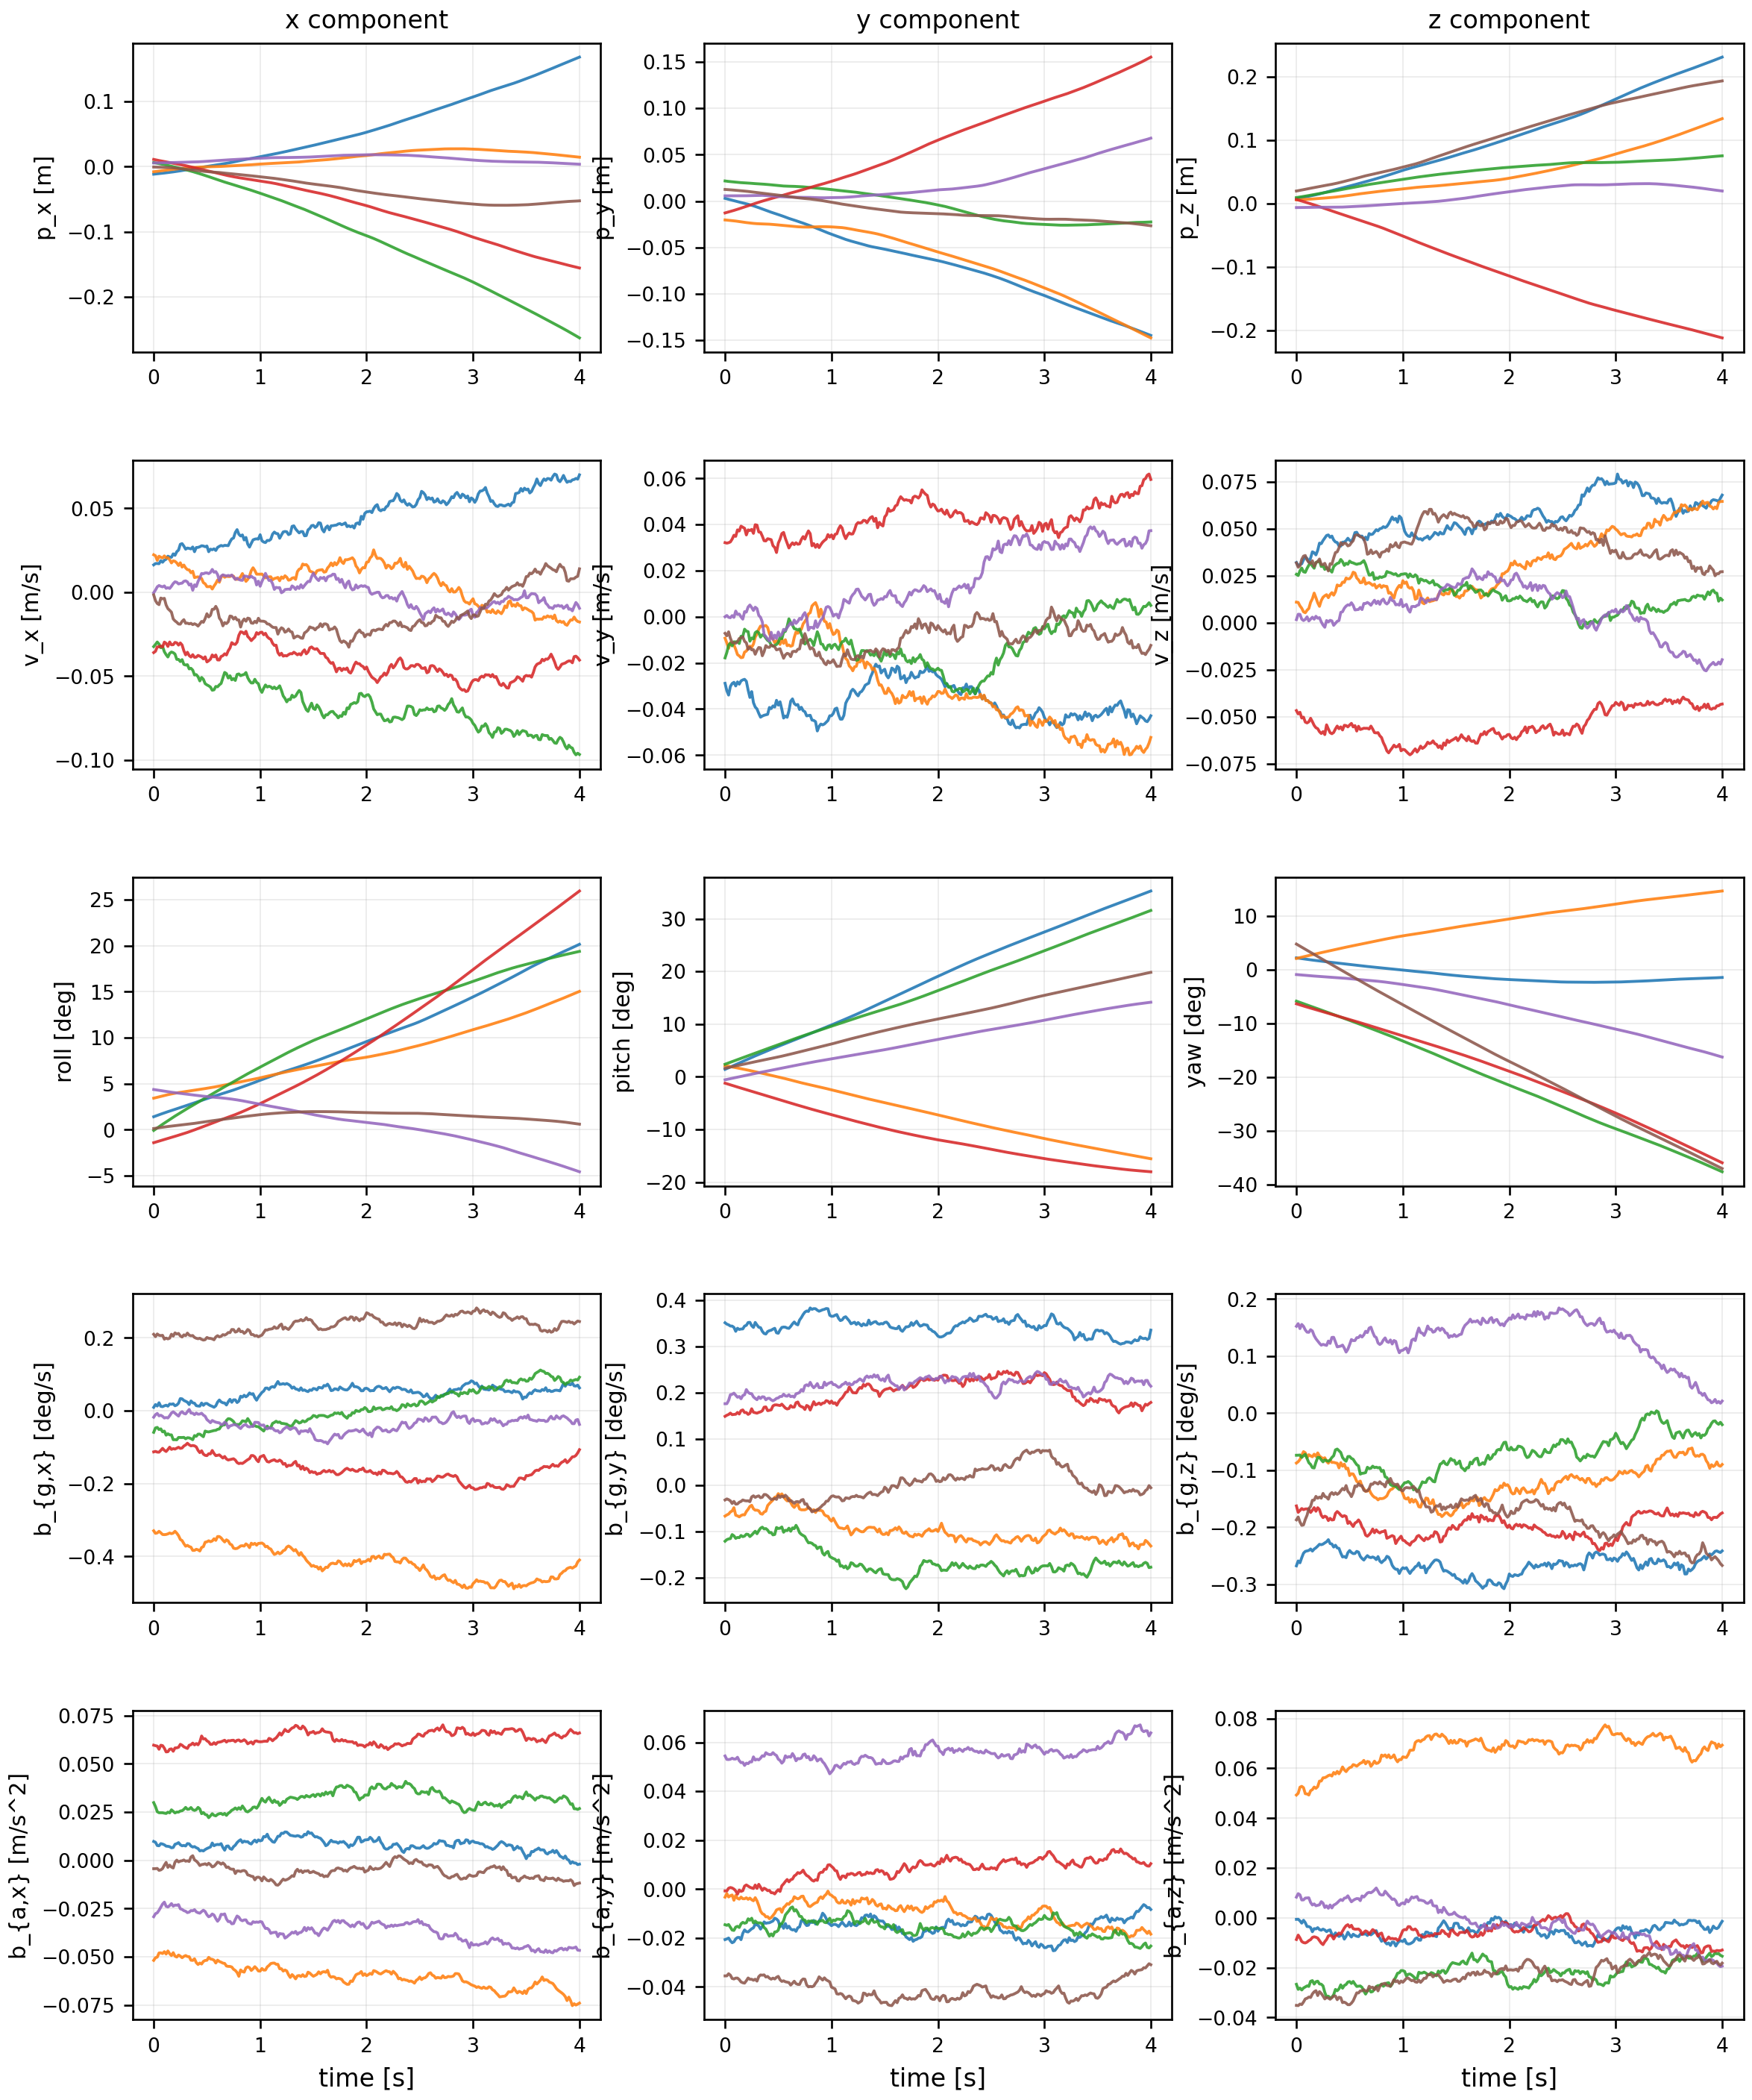
\includegraphics[width=\textwidth]{prior_state_evolution.png}
\caption{Evolution of all filter-state entries for six prior samples. The third row displays orientation through roll, pitch, and yaw angles for visualization only. In the actual Bayesian formulation, the orientation posterior is represented locally in tangent coordinates or through a quaternion-plus-error representation rather than by filtering Euler angles directly.}
\label{fig:prior_state_entries_annex}
\end{figure}

\section{How these samples should be interpreted}

The figures in this annex are useful because they connect the abstract prior hyperparameters to visible trajectory behavior.

\begin{itemize}
  \item Increasing $\sigma_a$ makes the translational paths rougher and increases position spread rapidly over time.
  \item Increasing $\sigma_\alpha$ makes the orientation process wander more aggressively.
  \item Increasing $\sigma_{bg,\mathrm{rw}}$ or $\sigma_{ba,\mathrm{rw}}$ produces visibly drifting bias traces, which later appear in the filter as slower but persistent nuisance evolution.
  \item Tightening the initial spreads $\sigma_{p0},\sigma_{v0},\sigma_{\mathrm{rpy},0}$ shrinks the cloud near the start of the sequence, but it does not remove dynamic uncertainty later in time.
\end{itemize}

This is exactly why the prior deserves as much attention as the likelihood. Before any measurements are assimilated, the prior already says what kinds of motion are considered plausible. In a Kalman filter or IEKF, the same assumptions reappear as the initial covariance and the process-noise matrices. In a fixed-lag smoother or factor graph, they reappear as Gaussian motion factors. In a path-space Bayesian formulation, they are the law that generates the random curve itself.


{\footnotesize\bibliographystyle{unsrtnat}\bibliography{references}}

\end{document}
